% Read This:
% Notation:
% ??? = unsure about something, some flaw in Text, something is missing
% !!! = there is still work to do here
%
% write Libraries like \texttt{PyTorch}



\documentclass[12pt]{article}

%\usepackage{biblatex}

\usepackage{graphicx}         % fuer das Einbinden von Grafiken
\usepackage{caption}       
\usepackage{comment}  
\usepackage{float}
\usepackage{subfigure}
\usepackage{amsmath}					%Um Formeln einzugeben
\usepackage{amssymb}					%Sonderzeichen und Symbole	
\usepackage{hyperref}
\usepackage{listings}
\usepackage[utf8]{inputenc}





\RequirePackage[backend=biber,
sorting=none, % http://tex.stackexchange.com/a/51439
maxcitenames=2]{biblatex} %% biber with biblatex
\DeclareFieldFormat{apacase}{#1} % disable case altering
\newrobustcmd{\citeright}[1]{\begin{flushright}-- \citeauthor{#1}, \citeyear{#1}\end{flushright}} % like \cite{} but with a dash and aligned to the right
\addbibresource{sources.bib}

\usepackage{siunitx}


% Title Page
\title{AML Final Project: Creating an Image Input Calculator} %Ullrich Köthe
\author{Timothy Jay Herbst, Fenja Kollasch, Duc Anh Phi}

\begin{document}
	\maketitle
	
	\begin{abstract}
		This paper discusses a program that can solve a variety of handwritten mathematical equations, using state-of-the-art computer vision and machine learning methods.
		Given a single image or a stream of images, the program is able to detect, recognize and compute written equations in real time.
		We came up with a series of steps to tackle this challenge.
		Initially, we remove noise with a preprocessing step.
		Then, each handwritten character is segmented from the image and its size, shape and positional information is used to infer its position in the equation.
		This also allows simple characters (e.g. points and bars) to be classified.
		The remaining characters are recognized using an \textit{AlexNet} Artificial Neural Network.
		Knowing the position and the class of the characters, allows us to reconstruct the equation as a string and pass it to the Symbolic Math Solver \texttt{SymPy}.
		By being open source this project demonstrates, how such a problem may be tackled and could give a basis for many other projects on a variety of topics.
		
		
		
	\end{abstract}
	\newpage
	
	\tableofcontents
	
	\newpage
	\section{Motivation}
	\small{Author: Timothy Jay Herbst} \newline \newline
	Computers are superior to humans in many everyday disciplines.
	A Calculator, for instance, can produce the solution to most simple mathematical problems faster than the user can enter it.
	This has inspired us to search for a solution to this flaw in a common household item.
	If we want to improve upon calculators, we will not have to increase the speed at which computers calculate.
	Instead the focus should lie on improving the efficiency of entering an equation into the calculator.\\
	We decided to make a calculator able to find the solution to an equation, when given an image of it.
	In this paper, we explain how such a calculator can be designed.\\ Similar projects have been successfully implemented \cite{inspired-blog}. Our project places its focus more on the complex task of using real and often noisy images.
	We hope that this serves as an inspiration to solve similar issues, and that the code provided proves useful.
	
	\section{Introduction}
		\small{Author: Fenja Kollasch, Duc Anh Phi} \newline \newline
	They way our brain solves handwritten formulae is similar to our program. We see the equation \texttt{(input)}, more specifically each character \texttt{(segmentation)} and recognize them as what they represent \texttt{(recognition)}. The focus is on what is written, so other things like the background are disregarded \texttt{(preprocessing)}. We skim over the equations from left, to right, top to bottom \texttt{(ordering)} and compute the result in our head along the way \texttt{(solving)}. Usually all the steps before finally computing the result, like segmentation and recognition are done effortlessly by our brain - the actual solving takes more time. Interestingly this phenomena is reversed with a machine. Calculations are rapid and easy to implement. However, reconstructing the written formula, by reading and interpreting visual information takes much more effort. It entails challenges in the areas of visual computing and machine learning.\\\\
	For once, several visual computing methods need to be applied to the image. The application has to segment the input image into one segment per character. These segments have to be put in an order which correctly represents the written formula. This ordering step is not trivial as there can be multiple lines of written equations with varying height and straightness. Each line can also contain fractions. They pose a problem, as their nominators and denominators could be assigned to the wrong line. Making things more complicated, fractions can be nested too.\\\\
	Machine learning methods can be applied for the recognition of each segmented character. Luckily, the recognition of handwritten symbols is a well-known problem that has been approached by various researchers before. LeCun et al \cite{lecun1998} for instance discussed different methods to recognized handwritten digits in 1998. With this work, they made a huge contribution by providing this MNIST database of handwritten digits \cite{mnist} that is used for many toy examples in machine learning. In fact, the task that is solved around the MNIST dataset does not differ very much from our own classification task. Symbols that can appear in a calculator input will mainly be digits from 0 to 9. Additionally, mathematical operators, brackets, latin symbols and greek symbols could be found in a mathematical formula. For this work however, we will focus on recognizing only digits and simple mathematical operators like plus, minus, multiplication-, and division symbols, as well as brackets.\\\\
	After these steps are completed, we end up with a reconstructed formula which we pass to a symbolic math solver, in our case \texttt{SymPy}, which is an open source python library. We then present the recognized equations with the computed results.\\\\
	We implemented the program to harnesses the local webcam and use the stream of frames as the input. The whole process of preprocessing, segmenting and ordering each frame is computed and displayed in near real-time.
	The whole application flow is summarized in the figure below:
	\begin{figure}[h]
		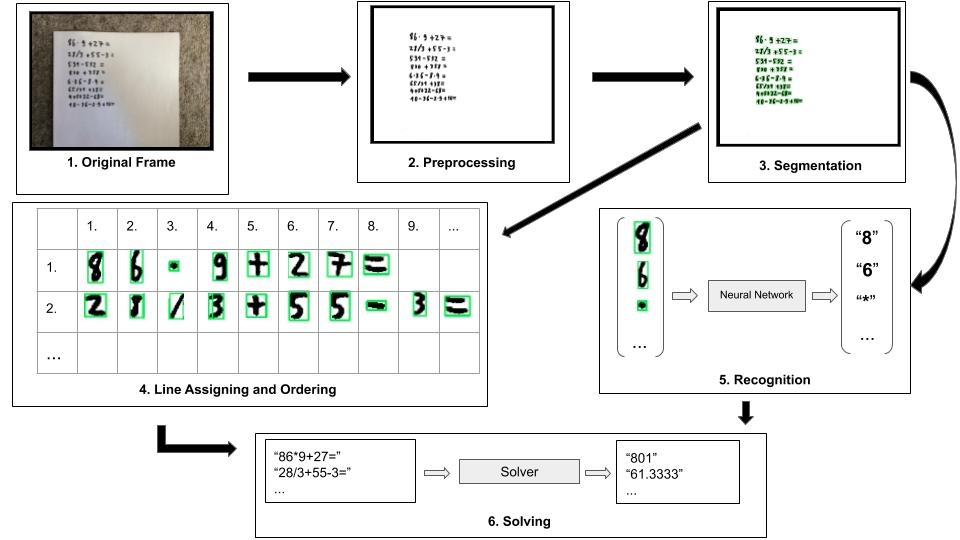
\includegraphics[width=1\textwidth]{ImagesForReport/fulldiagram.jpg}
		\caption{Application Flow}
		\label{fig:FullFlow}
	\end{figure}

	\addtocontents{toc}{\protect\setcounter{tocdepth}{1}}
	\pagebreak\section{Previous work}
	As mentioned in the introduction, we are approaching a number of common problems in computer science. Therefore, an amount of related work exists. The motivation of this report declares that we took inspiration of a blog post \cite{inspired-blog} proposing an application with a similar workflow. 
	
	The recognition of handwritten symbols beyond digits has received attention as well. Shortly after the introduction of MNIST, the data set was extended to EMNIST \cite{emnist} including not only digits, but also handwritten characters. Meanwhile, one can find various data sets with handwritten symbols, even specialized on mathematical symbols \cite{chajri2016}. There are existing Kaggle challenges for solving this classification issue \cite{kaggle} which as a rich amount of solutions. So far, there have been many approaches on the topic by using machine learning as we did \cite{ramadhan2016} \cite{lee2016}. Additionally, there are different approaches where the classification of the symbols succeeds over the geometrical properties of the symbols \cite{golubitsky2010}. 
	
	\section{Theory}
	\subsection{Classification with neural networks}	
	The state-of-the-art for automatically recognizing the content of an image file is to solve this issue with \textit{artificial neural networks}. In theory, this design pattern bases on the neuron structure of the human brain as described by neuroscientists. According to this concept, a neural network consists of different layers with a certain amount of nodes which are also referred to as \textit{neurons}. Each neuron receives an input of different parameters that either come from the previous neuron layer or they are given as initial input. A non-linear function is applied to this input that creates an output value. This value is lead to the next layer where it acts as an input again. The first layer of a neural network is often referred to as the \textit{input layer}, while the last layer is called the \textit{output layer}. Between these layer lies a freely chosen number arbitrarily large \textit{hidden layers} (see figure \ref{fig:simple-nn}).
	
	\begin{figure}[h!]
		\centering
		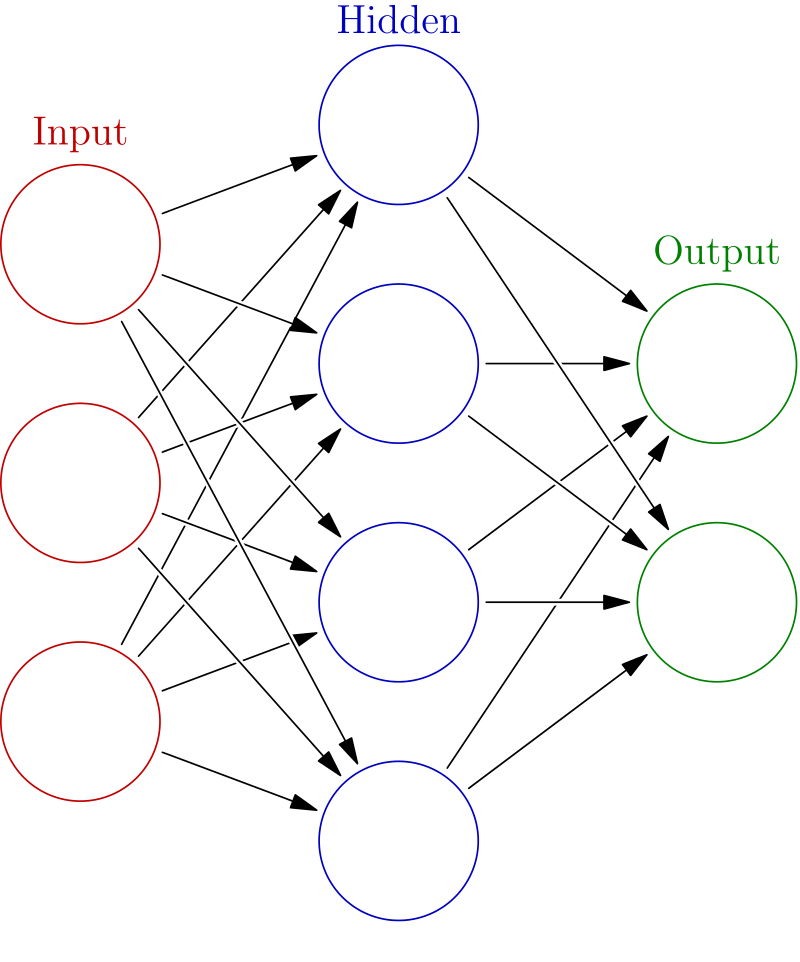
\includegraphics[width=0.5\textwidth]{ImagesForReport/simple-nn.png}
		\caption{A simple artificial neural network}
		\label{fig:simple-nn}
	\end{figure}
	
	Classifying an image means to have a neural network predict how likely the image shows an object from an acquainted catalog, so-called \textit{labels}. As an input, the neural network receives an array including this image's color values. Therefore, the amount of neurons in the input layer needs to be conform with the size and the number of color channels of the input image. The first layer will now produce a certain number of output values that are passed to the next layer. How many output values are generated and to which neurons of the next layer they are passed, depends on the network architecture. When the input meets the last layer of the network, the output layer will calculate for each known label the probability on which the image displays something that can be described with this label. This means, the final output of the network is a vector mapping the probabilities to the known labels. To make a distinct classification of the image content, one would assign the label with the highest probability to the image. Furthermore, it is also possible to design a network that takes not only a single but a set of images as an input and predicts labels for all images. Thus, it will not return a vector with probabilities, but a matrix.
	
	The just described \textit{forward pass} is used to make a label prediction for an input. However, if data is lead through an untrained network, the prediction is no better then a guess. To make a reliable network, it is necessary to \textit{train} it, usually by passing a high amount of labeled images and comparing the predictions to the labels. The error calculated through the difference between prediction and ground truth now gets \textit{backpropagated} through the network by regarding the gradient at the previous neurons and adapting the weights at the neuron's cost function to minimize the error. This is an iterative process, which is why a training cycle usually has multiple \textit{epochs} where the whole training data set is passed forward and backward. Furthermore it has been proven beneficial to not lead the whole set at once through the network, but to take smaller batches that include randomly chosen samples from the training set. There are various optimization algorithms for the backward pass, as well as different metrics to estimate the error between ground truth and prediction.

	\subsection{Adaptive Threshold} %??? !!! Add before vs after Images, after Preprocessing is complete
	\small{Author: Timothy Jay Herbst} \newline \newline
	A problem we face with the images, is that we do not know if a pixel is part of the writing or not.
	The "Adaptive Threshold" function \cite{adaThresh}, found in the \texttt{OpenCV} library is very useful in this case. %???
	This function operates like most threshold functions, in that it compares a pixel to a threshold $T$.
	If the pixel is found to have a value higher than the threshold $T$, we set it to 255.
	Otherwise the pixel is set to a value of 0 \cite{cvAdaThresh}
	%		\begin{align}
	%			newImg(x,y)=
	%			\left
	%			\begin{cases}
	%			255  \hspace{1cm}&\mathrm{if} \hspace{0.5cm} img(x,y)>T \\
	%			0  &\mathrm{else}
	%			\end{cases}
	%			\right.
	%		\end{align}
	This way it is possible, to easily "classify" a pixel as writing (0) or not (255).\\
	What makes this function work so well, is that for every pixel the threshold $T(x,y)$ is calculated separately.
	While there are several different ways, how we can calculate this, it was found to work best for our problem, by a simple process [2]:\\
	The threshold $T(x,y)$ is set to the gaussian weighted sum of every pixel within a window with side length 11 (extends 5=(11-1)/2 pixels out from (x,y)):
	\begin{align}
	T(x,y)=&\sum_{\Delta x=-5}^{5}\sum_{\Delta y=-5}^{5} -2 + G_{(\Delta x,\Delta y)} \cdot img(x+\Delta x,y+\Delta y)\\
	\mathrm{with}& \hspace{1cm} G_{(\Delta x,\Delta y)} = \alpha \cdot \mathrm{exp}(-(\Delta x ^2 +\Delta y^2)/(2*\sigma)^2)\\ %??? check
	&\mathrm{with} \hspace{1cm}\alpha = 1/\Big(\sum G_{(\Delta x,\Delta y)}\Big)\\
	&\mathrm{with} \hspace{1cm}\sigma = 0.3 \cdot ((11-1)/2-1) + 0.8 = 2
	\end{align}
	Here $\alpha$ is the normalisation factor and $\sigma$ is the  standard deviation (recommended by \texttt{OpenCV}) for a box size of 11.\\
	The values mentioned above were found to work well with most of the images tested.
	If a particularly large or small image would be tested, we would need to adapt these values
	%??? maybe add this	\subsection{Small Contour Filter Mask}
	
	
	\addtocontents{toc}{\protect\setcounter{tocdepth}{2}}
	\section{Design of the Image Input Calculator}
	
	\subsection{Data Collection}
	\small{Author: Timothy Jay Herbst} \newline \newline
	The user can have the program analyse images from a variety of sources.
	The library \texttt{OpenCV} is capable of reading image files, video files and may also use a webcam, if present.
	This enables a smooth user experience and allows realtime analysis of an equation.
	
	
	%Our program evaluates images.
	%The input source could be an image file, a video file or the local webcam.
	%We enable a smooth user experience as results are computed rapidly through efficient implementation.
	%The user could hold a sheet of written equations in front of the webcam and see the computed results almost immediately.
	
	\subsection{Preprocessing}
	\small{Author: Timothy Jay Herbst, Duc Anh Phi} \newline \newline
	Our program receives the original unaltered image.
	It is difficult to detect significant features, such as the symbols that make up the equation from such an image.
	Therefore, it is necessary to do some preprocessing, before further steps make sense.\\
	This raises several issues.
	Some improvements we could make include:\\
	\begin{itemize}
		% !!!
		\item Correction for different quality of camera, lighting, etc.:
		The incoming images vary significantly due to changes of lighting and may come from different cameras.
		Correcting for this, is not a simple task.
%		A future improvement of this project would improve greatly by having an adaptive preprocessing step.
		% !!!
		\item Simplification of the input dimensions: Explicitly we want our image to be a binary black-white image, with the colours black (0) and white (255).
		\item Connectedness of the symbols: For later steps, it is useful to not segment any symbols. In the same manner, we do not wish for two different symbols to be connected.
		\item Removal of noise: Often the background (e.g. paper or whiteboard) is not uniform and this can create spots in the image. (The human eye is very good at filtering these out.)
		\item Background contour removal: Oftentimes when taking an image of a contour there will be other objects in the image (e.g. pencils, the border of the paper, etc.).
		\item Correction for reflected bright spots: Especially, when using images from white boards, the program has to contend with reflected light sources.
	\end{itemize}
		%!!! ??? Add more
		We correct for (most of) these issues in three separate steps:\\
		First we use a few select image processing steps to deal with most of the issues.
		In a second step, we remove the contours that can be attributed to background objects.
		Lastly, we correct for reflected light sources. %!!! Add to master

	\subsubsection{Simple Preprocessing}%??? !!! Add stepwise Images, after Preprocessing is complete
	\small{Author: Timothy Jay Herbst} \newline \newline
	\begin{figure*}[htp]
		\centering
		\subfigure[Original Frame]{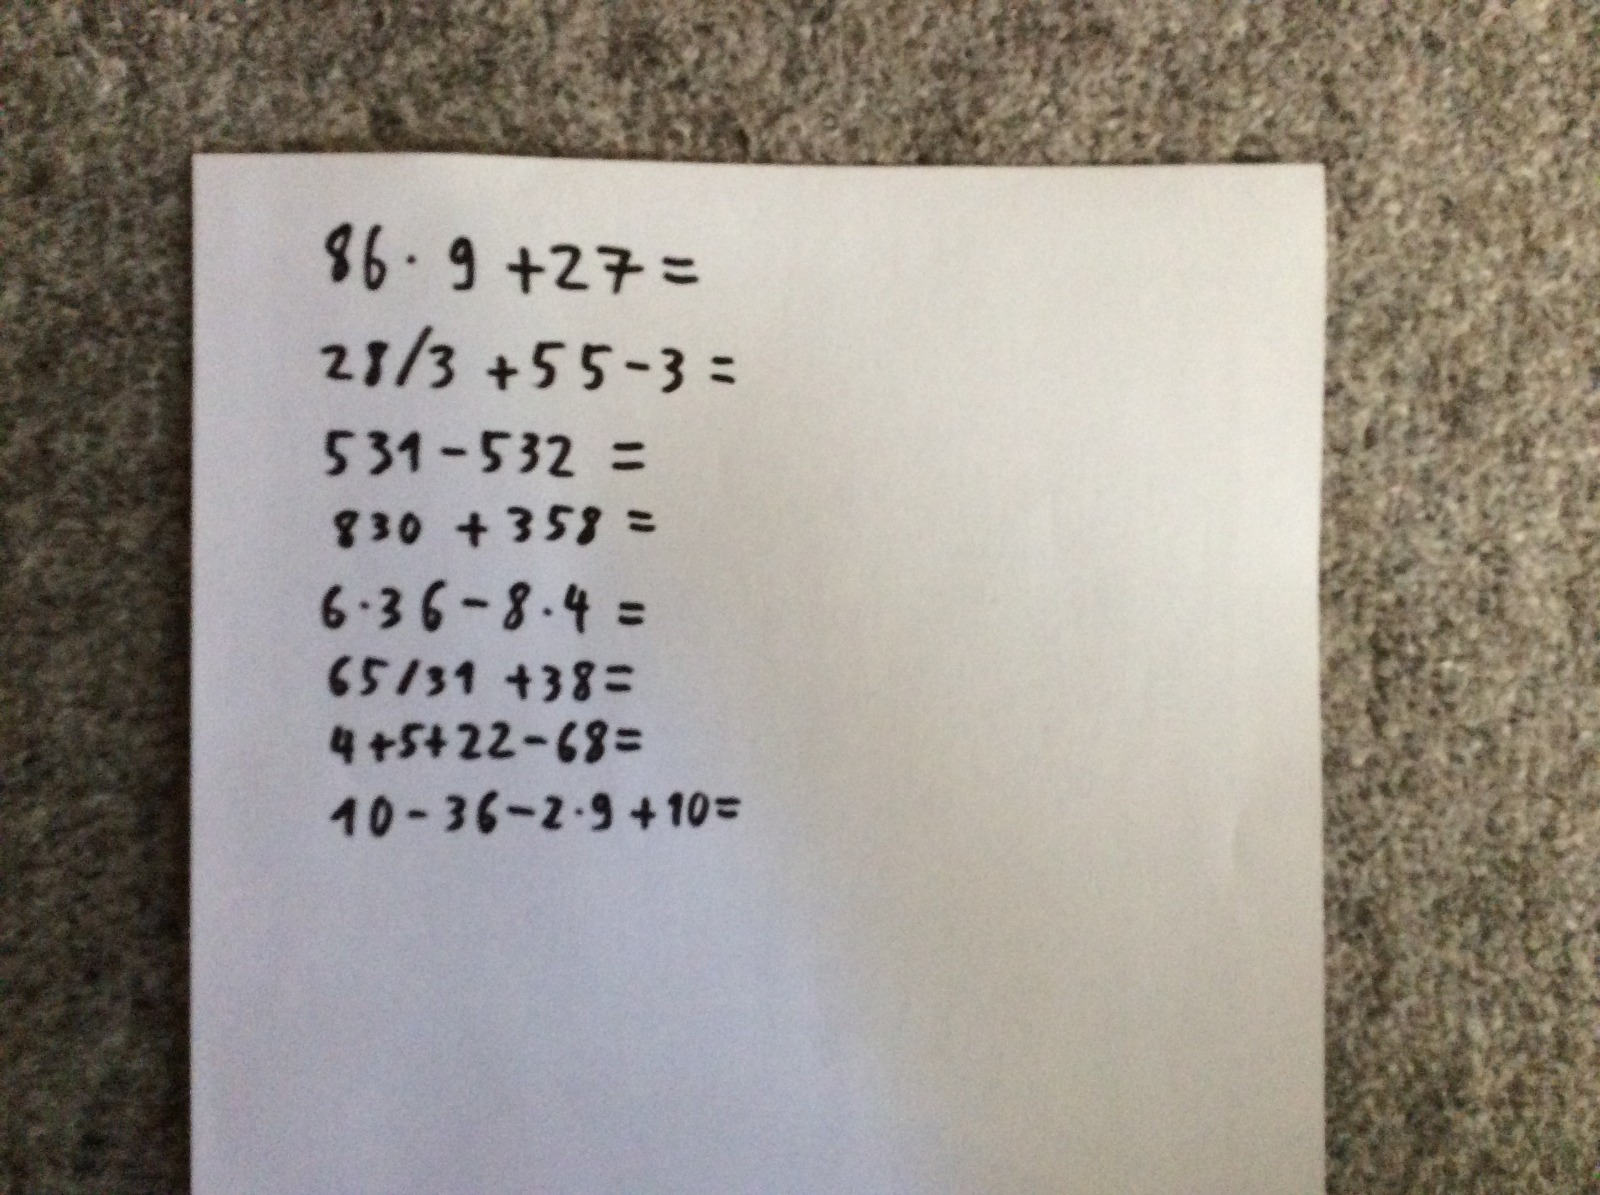
\includegraphics[width=.45\linewidth]{ImagesForReport/Frame}}\quad
		\subfigure[Grayscaled]{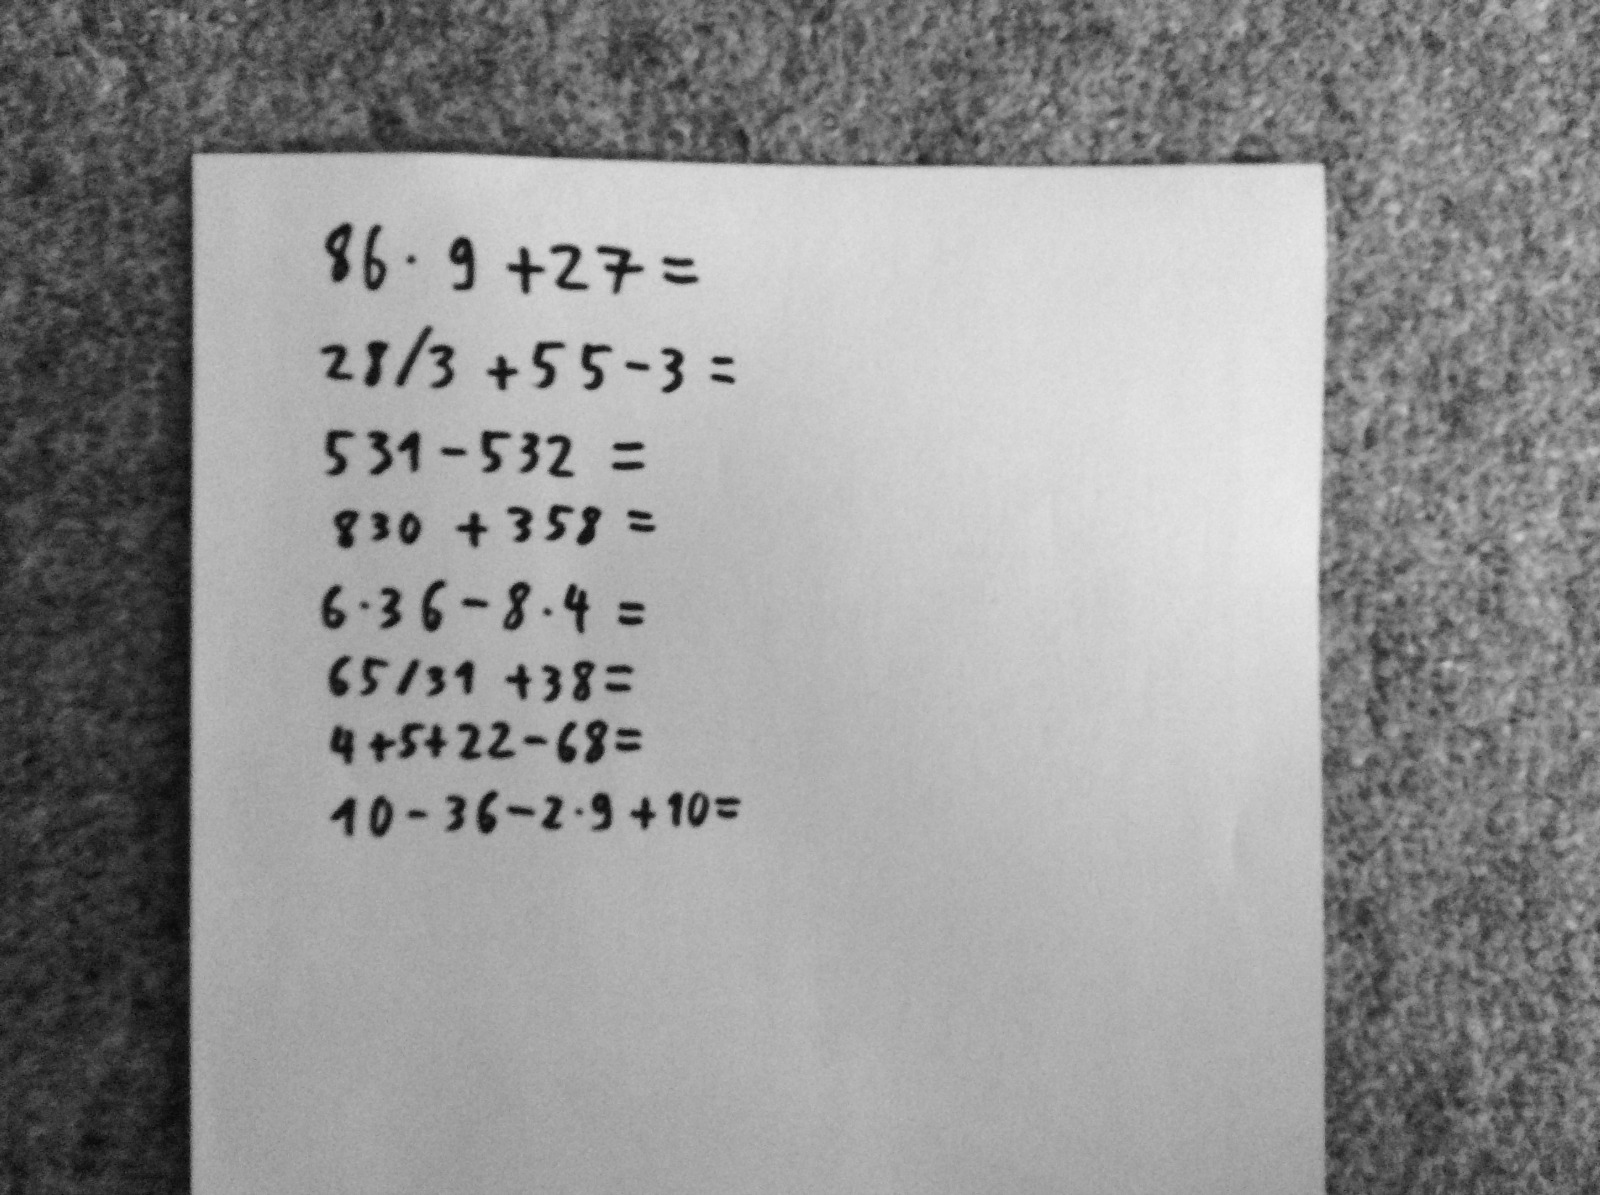
\includegraphics[width=.45\linewidth]{ImagesForReport/Grayscale}}
		
		\subfigure[Gaussian Blur]{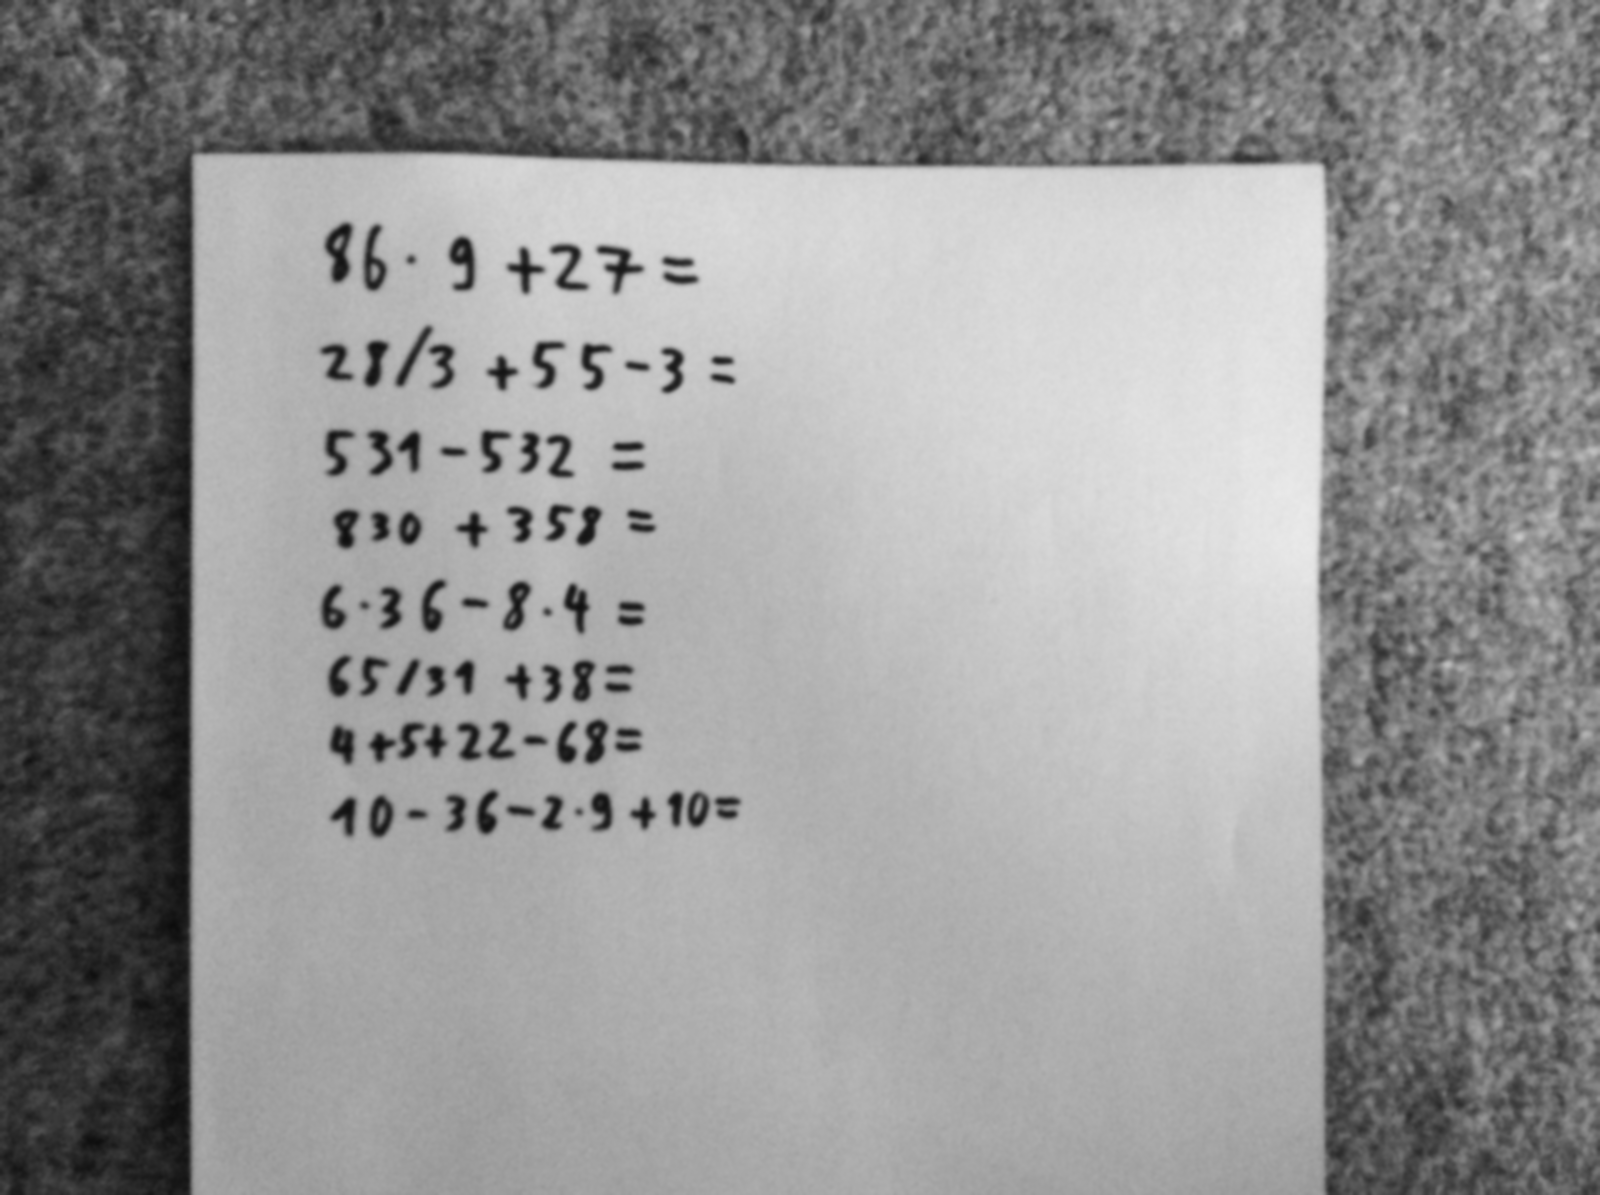
\includegraphics[width=.45\linewidth]{ImagesForReport/GaussianBlur}}\quad
		\subfigure[Morphological Opening]{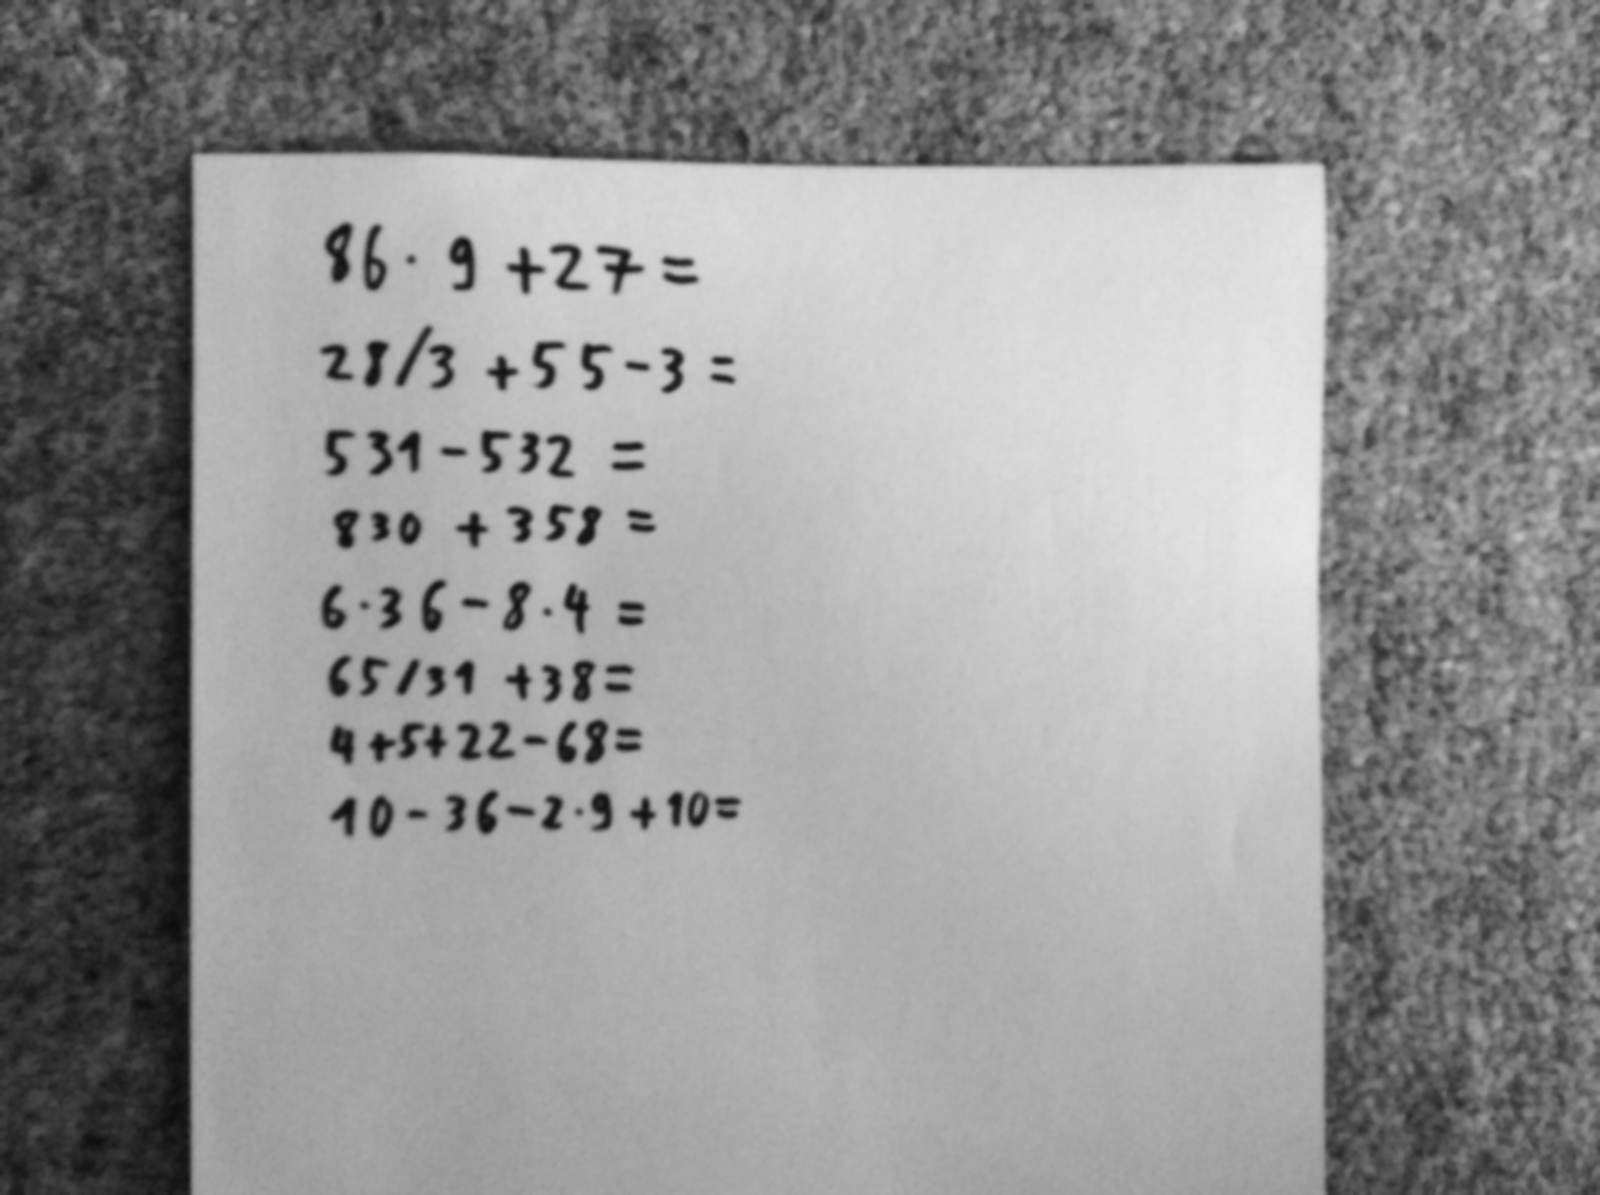
\includegraphics[width=.45\linewidth]{ImagesForReport/MorphOpen}}
		
		\subfigure[Adaptive Gaussian Thresholding]{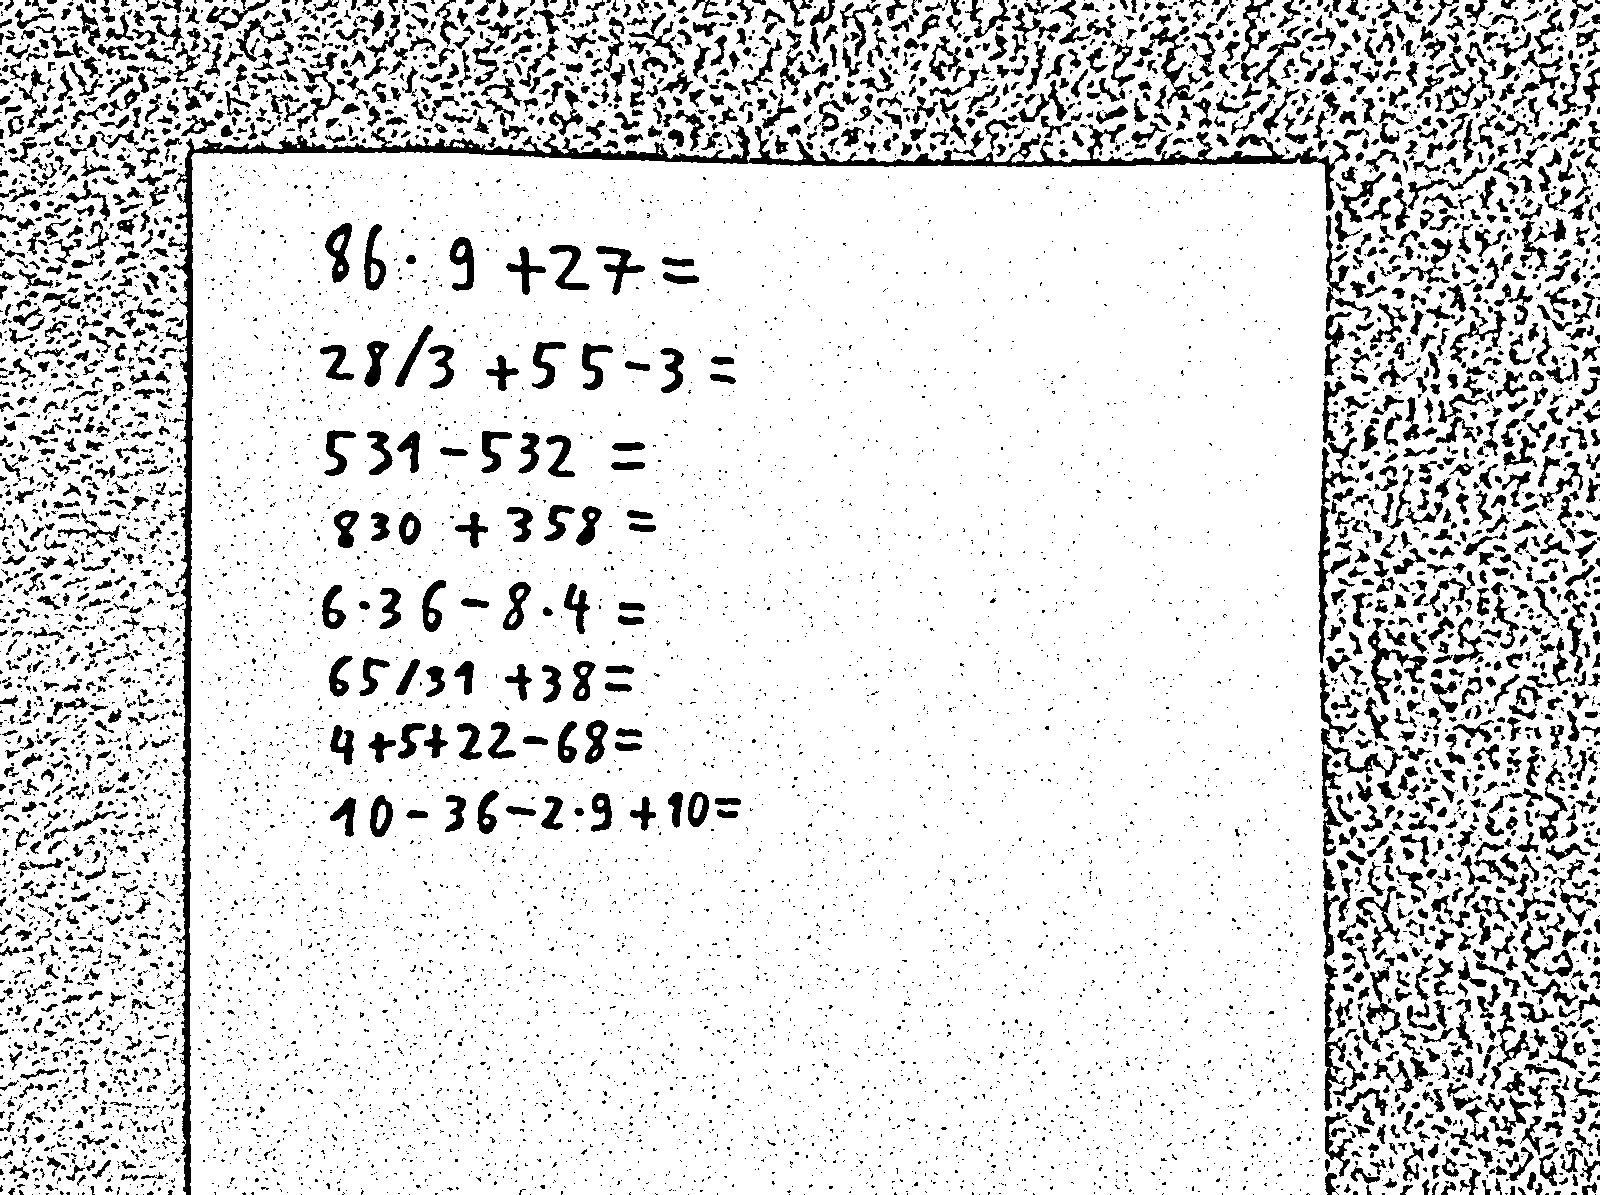
\includegraphics[width=.45\linewidth]{ImagesForReport/AdaptiveGaussianThresholding}}\quad
		\subfigure[Dilation]{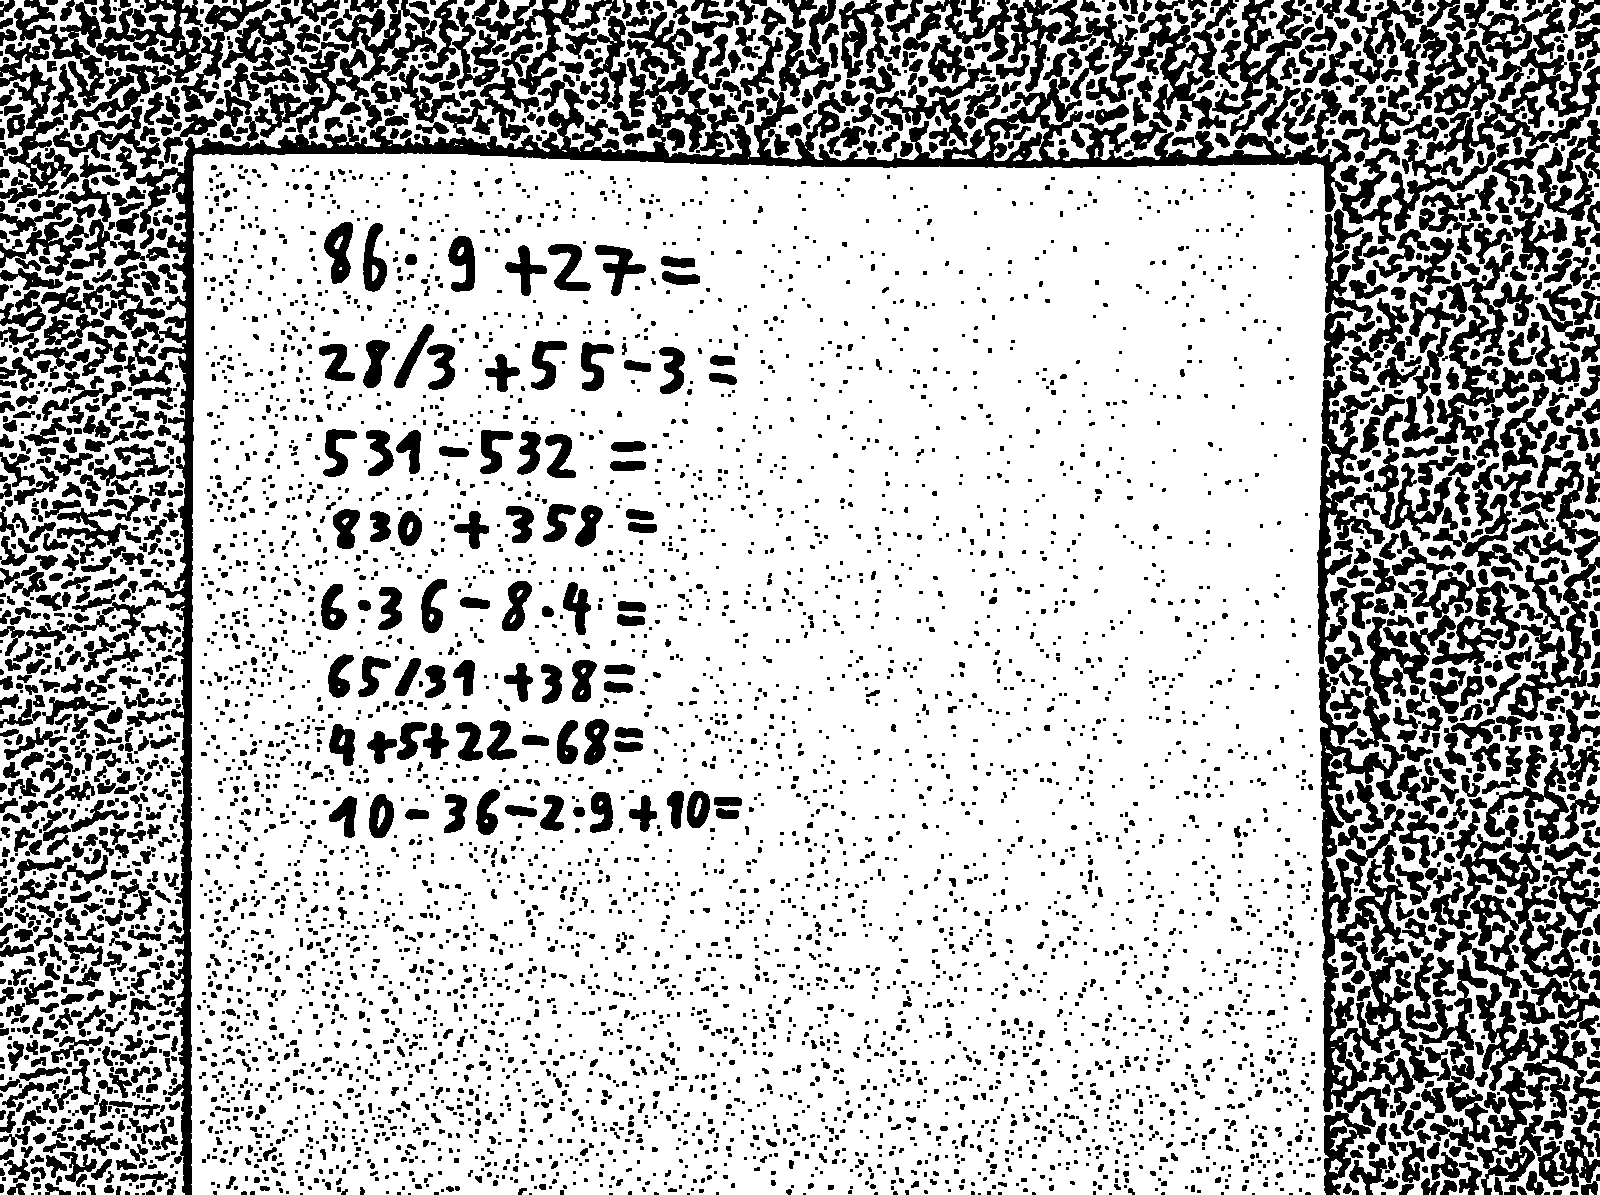
\includegraphics[width=.45\linewidth]{ImagesForReport/Eroding}}
		
		\caption{Various steps performed during the simple Pre-Processing Process}
		\label{fig:SimplePreprocessing}
	\end{figure*}

%	\begin{figure}
%		\centering
%		\begin{subfigure}{.5\textwidth}
%			\centering
%			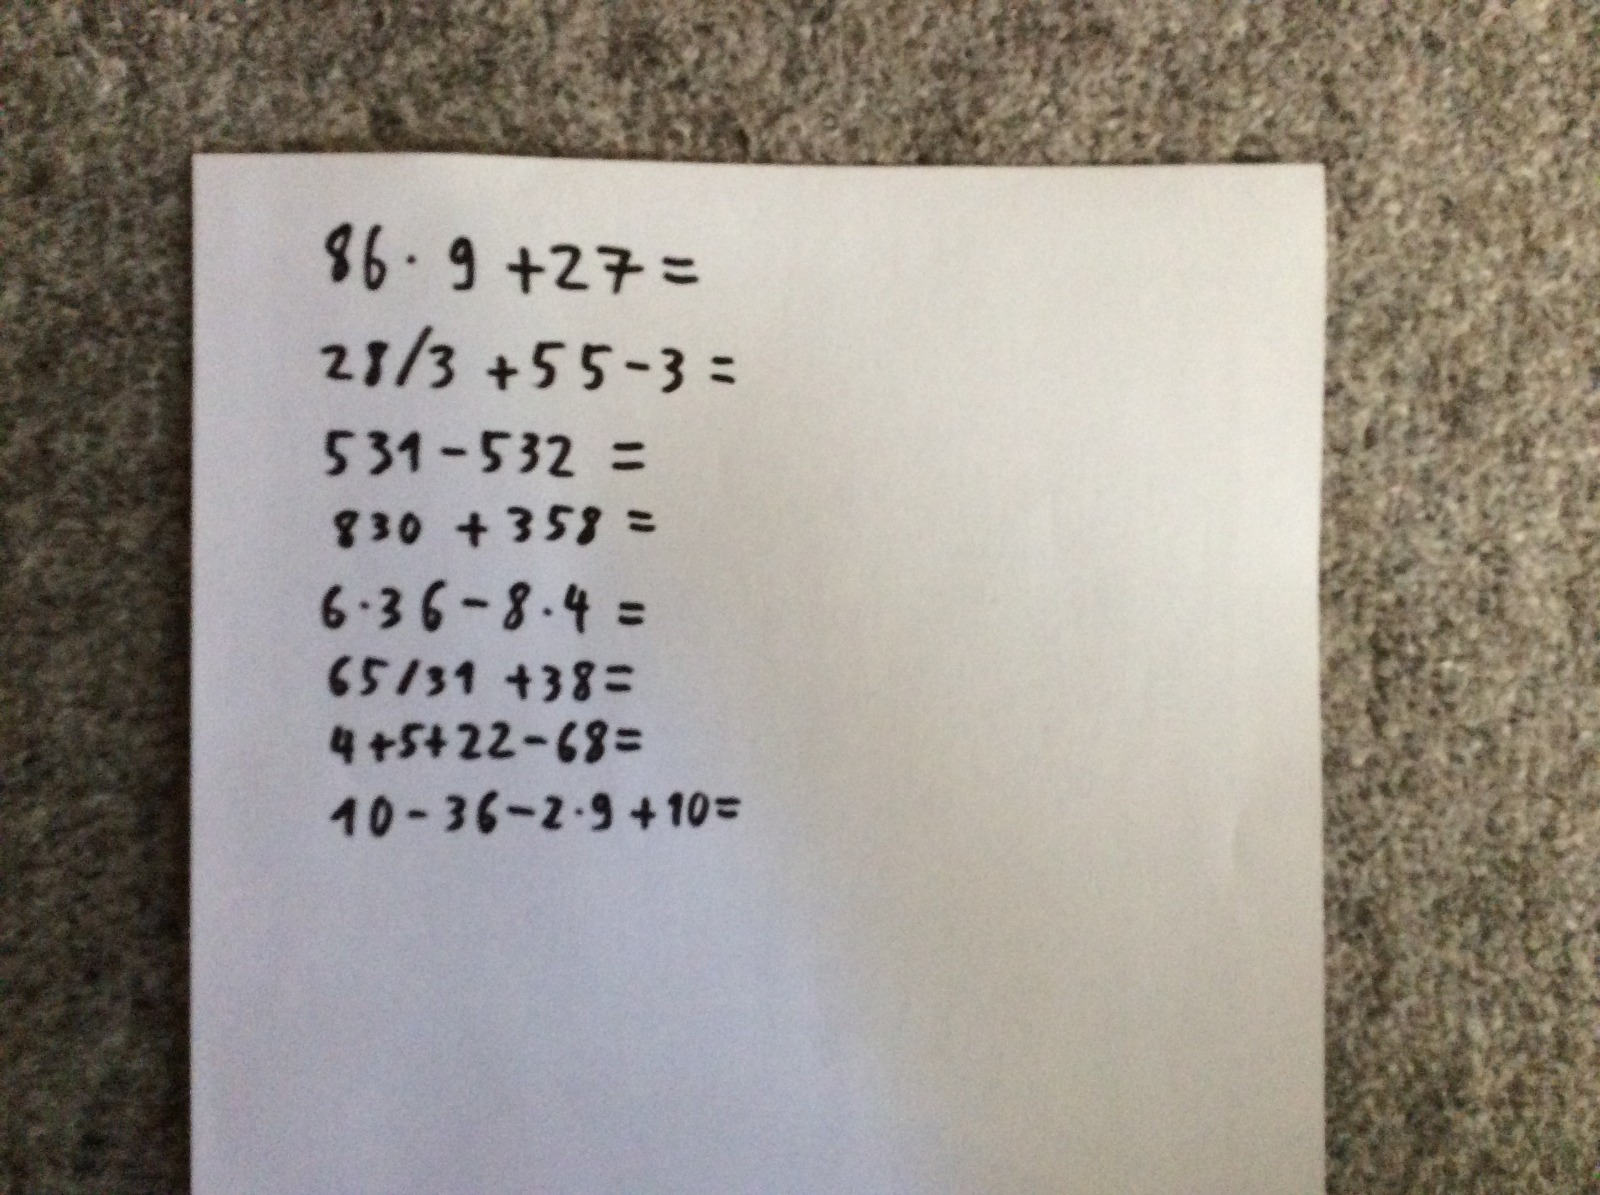
\includegraphics[width=.8\linewidth]{ImagesForReport/Frame}
%			\caption{Original Frame}
%			\label{fig:OriginalFrame1}
%		\end{subfigure}
%		
%		\begin{subfigure}{.5\textwidth}
%			\centering
%			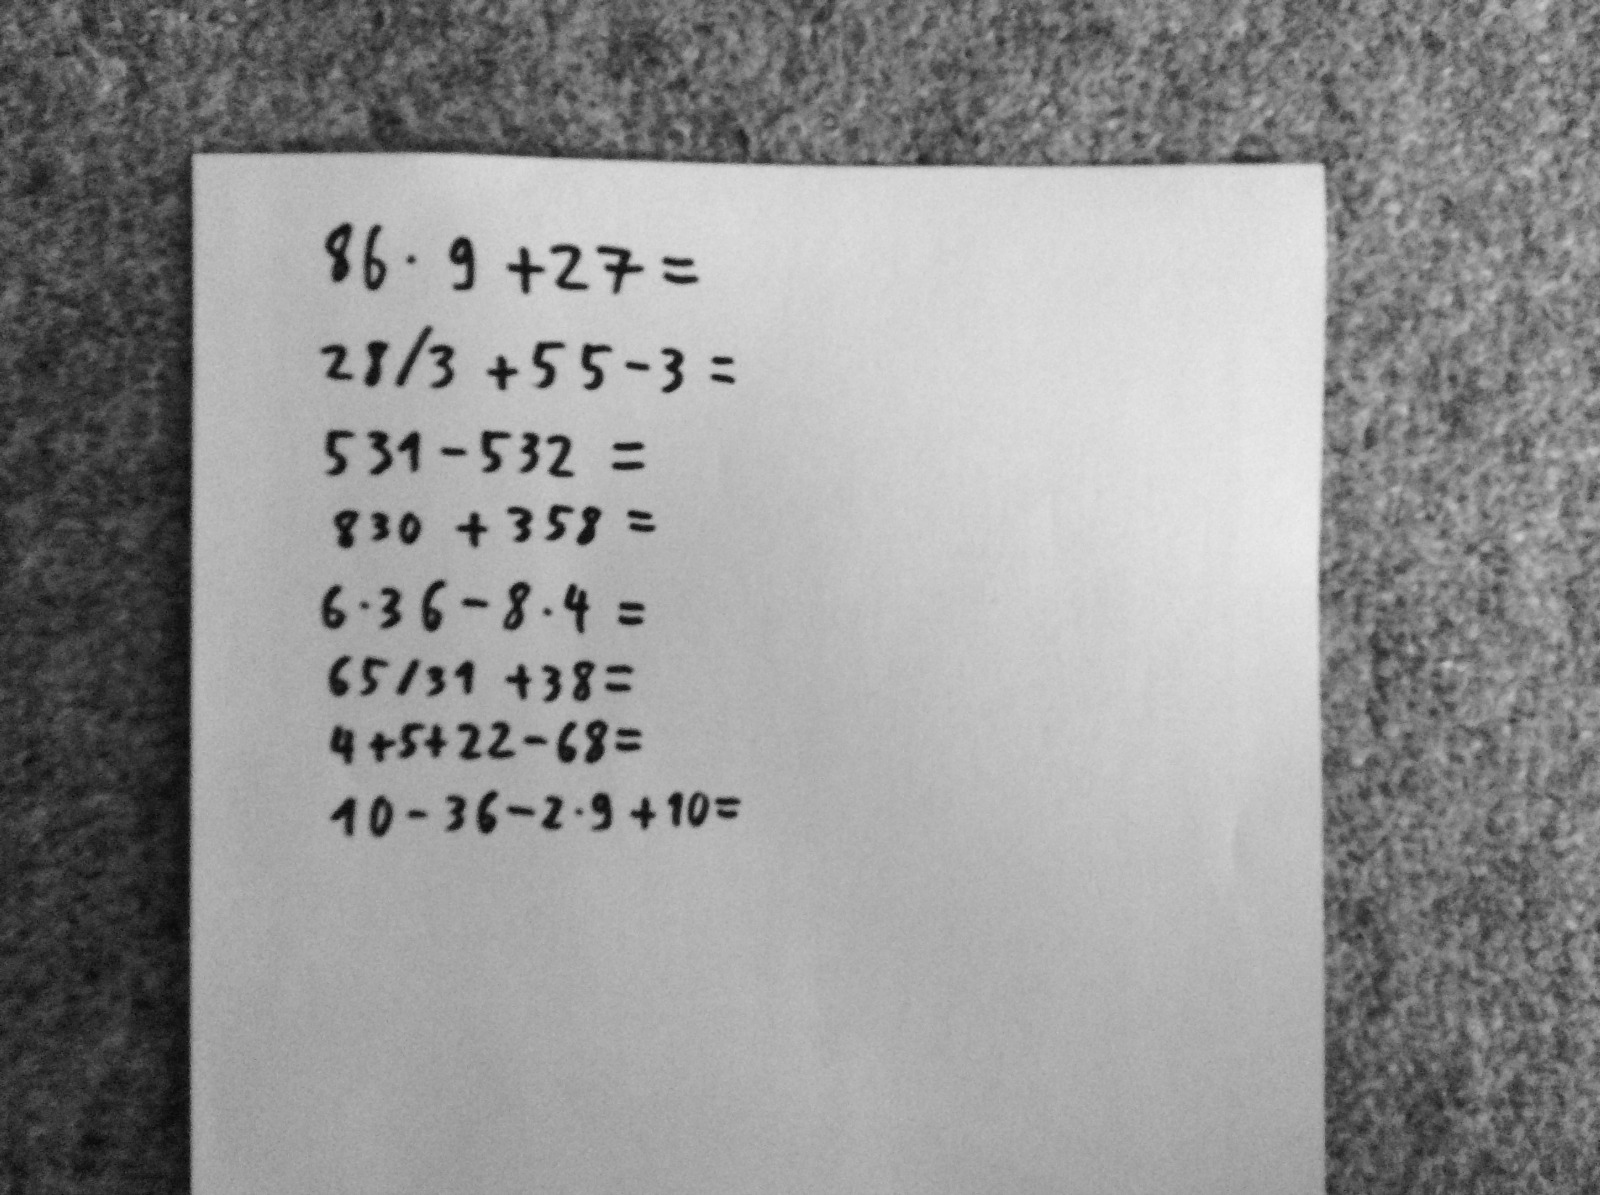
\includegraphics[width=.8\linewidth]{ImagesForReport/Grayscale}
%			\caption{Grayscaled}
%			\label{fig:Grayscale1}
%		\end{subfigure}\\
%		
%		\begin{subfigure}{.5\textwidth}
%			\centering
%			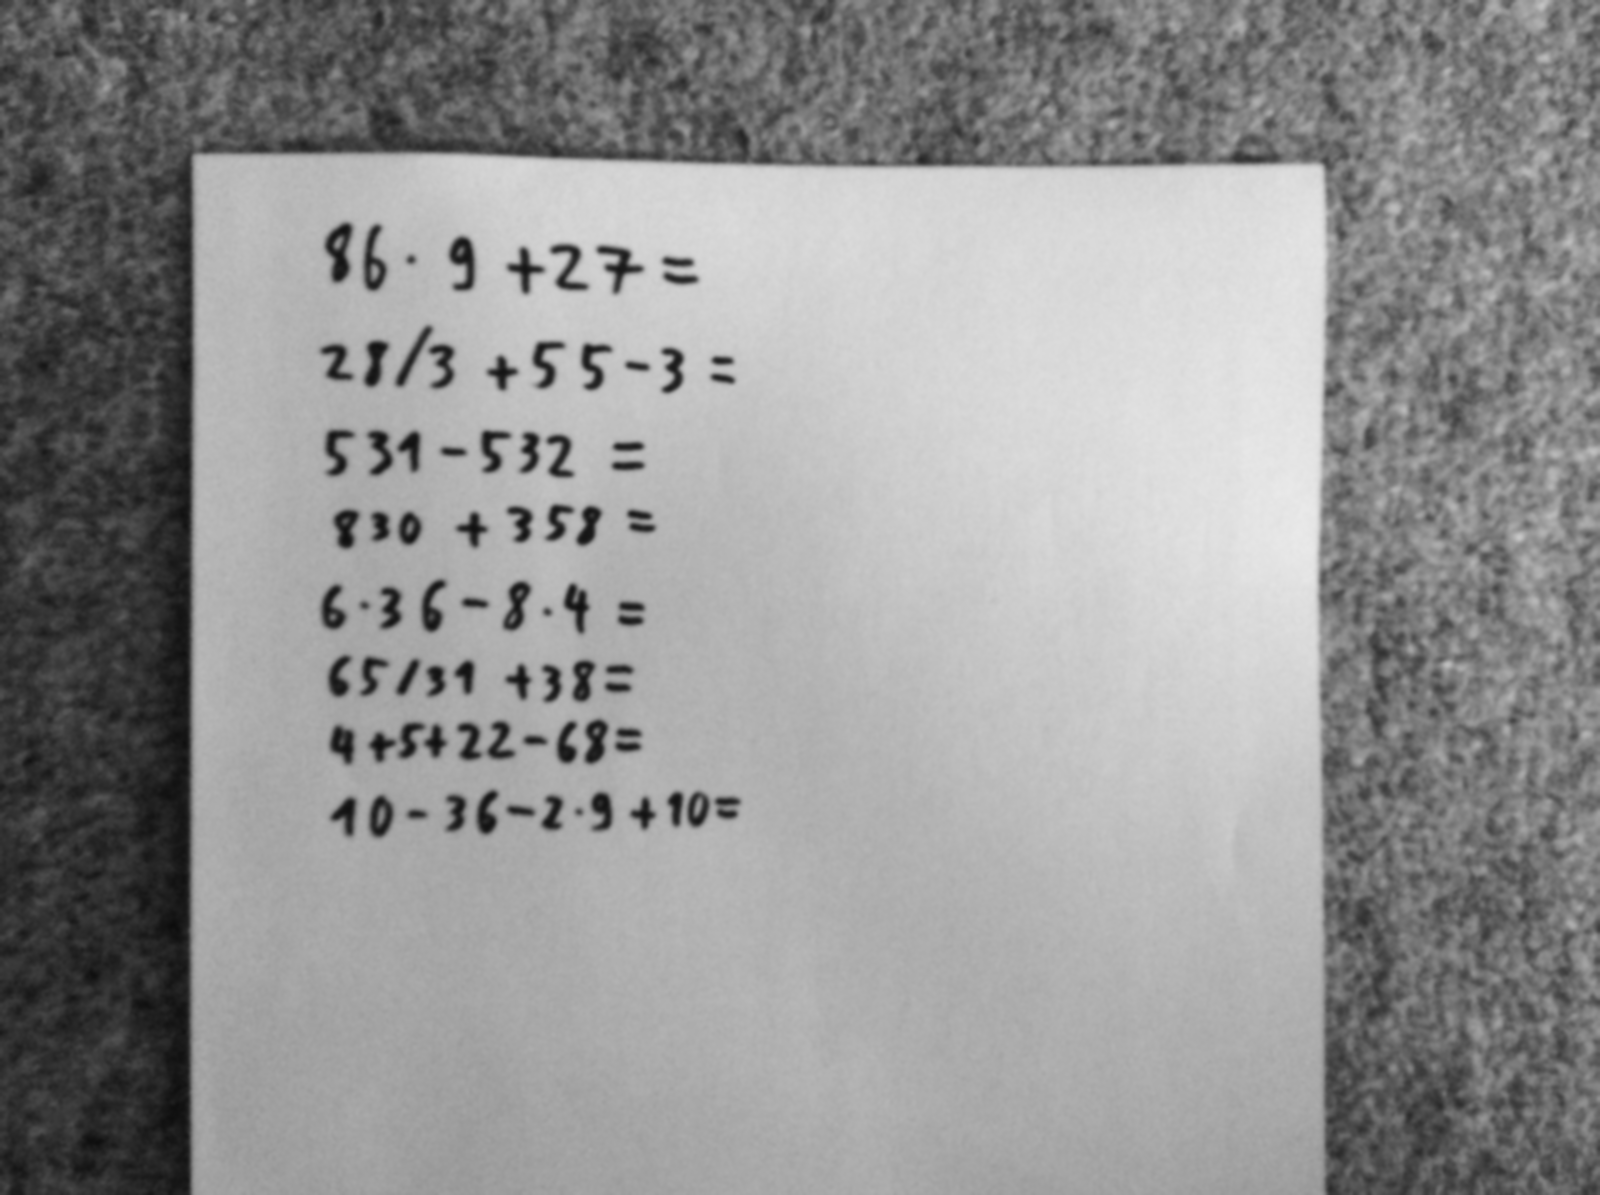
\includegraphics[width=.8\linewidth]{ImagesForReport/GaussianBlur}
%			\caption{Gaussian Blur}
%			\label{fig:GB1}
%		\end{subfigure}
%		
%		\begin{subfigure}{.5\textwidth}
%			\centering
%			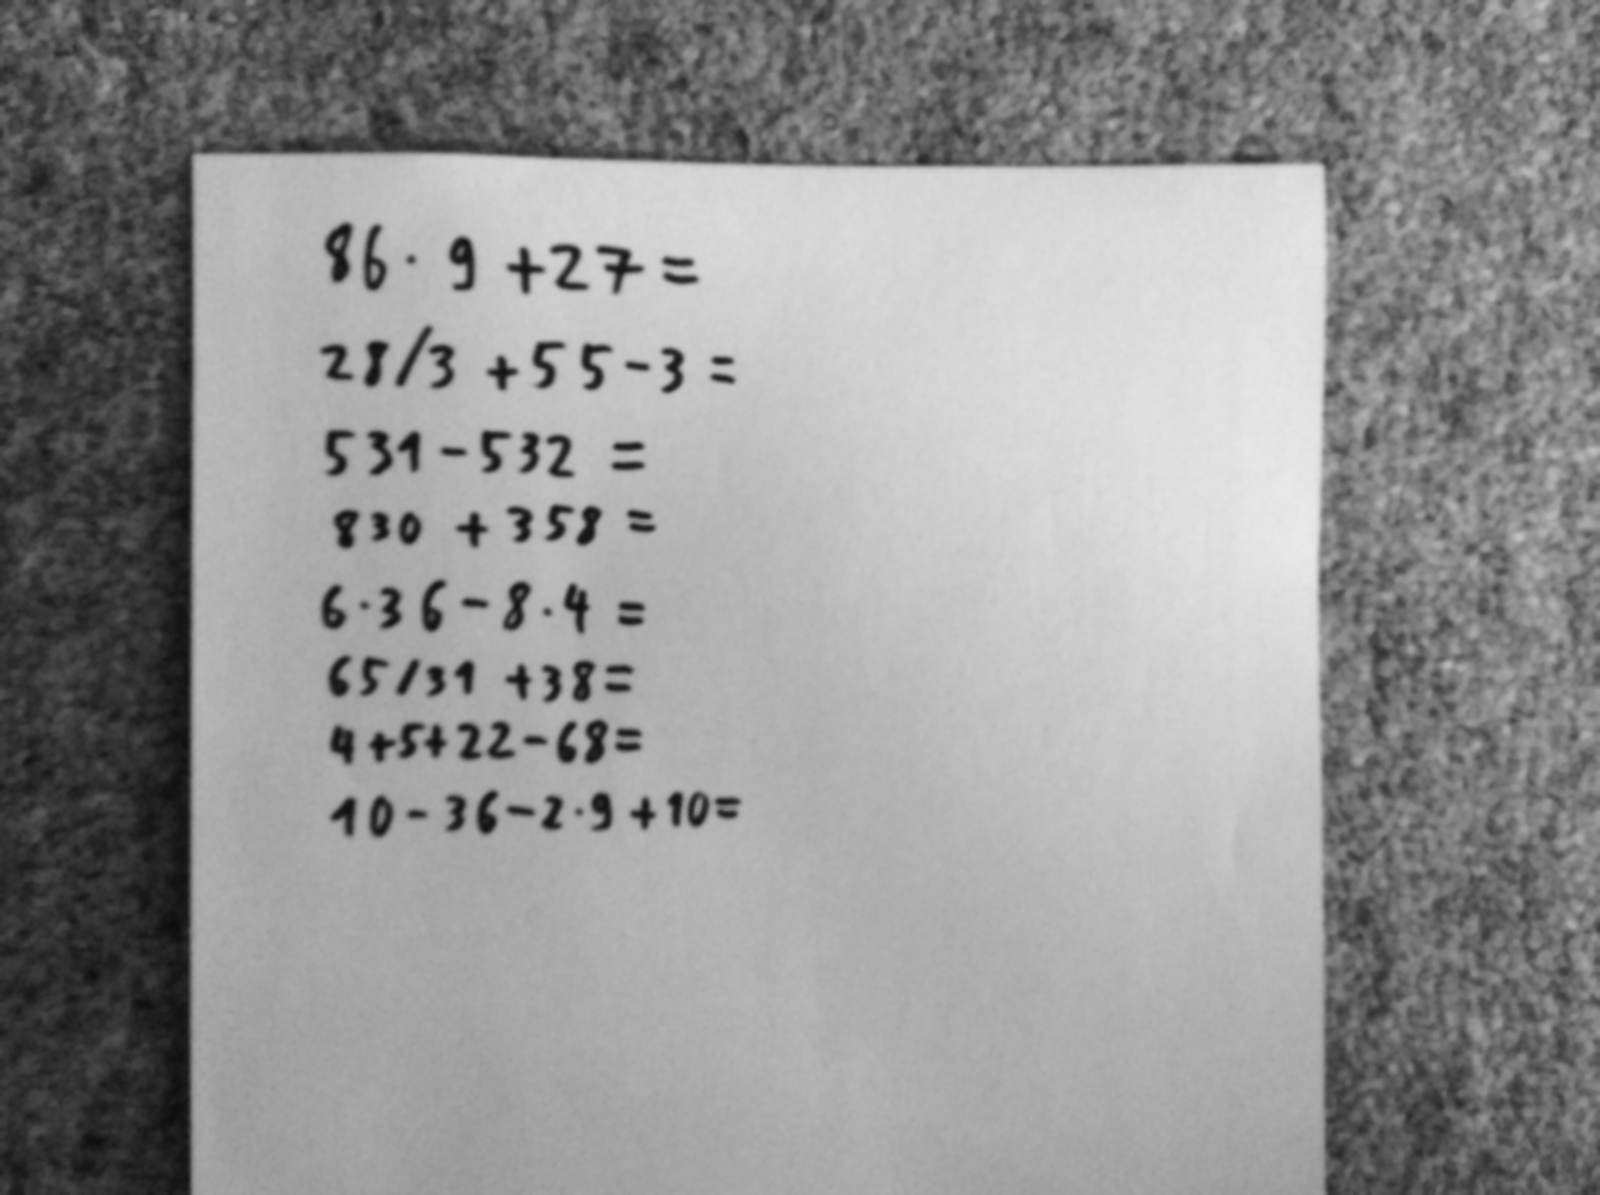
\includegraphics[width=.8\linewidth]{ImagesForReport/MorphOpen}
%			\caption{Morphological Opening}
%			\label{fig:MorphOpen1}
%		\end{subfigure}\\
%	
%		\begin{subfigure}{.5\textwidth}
%			\centering
%			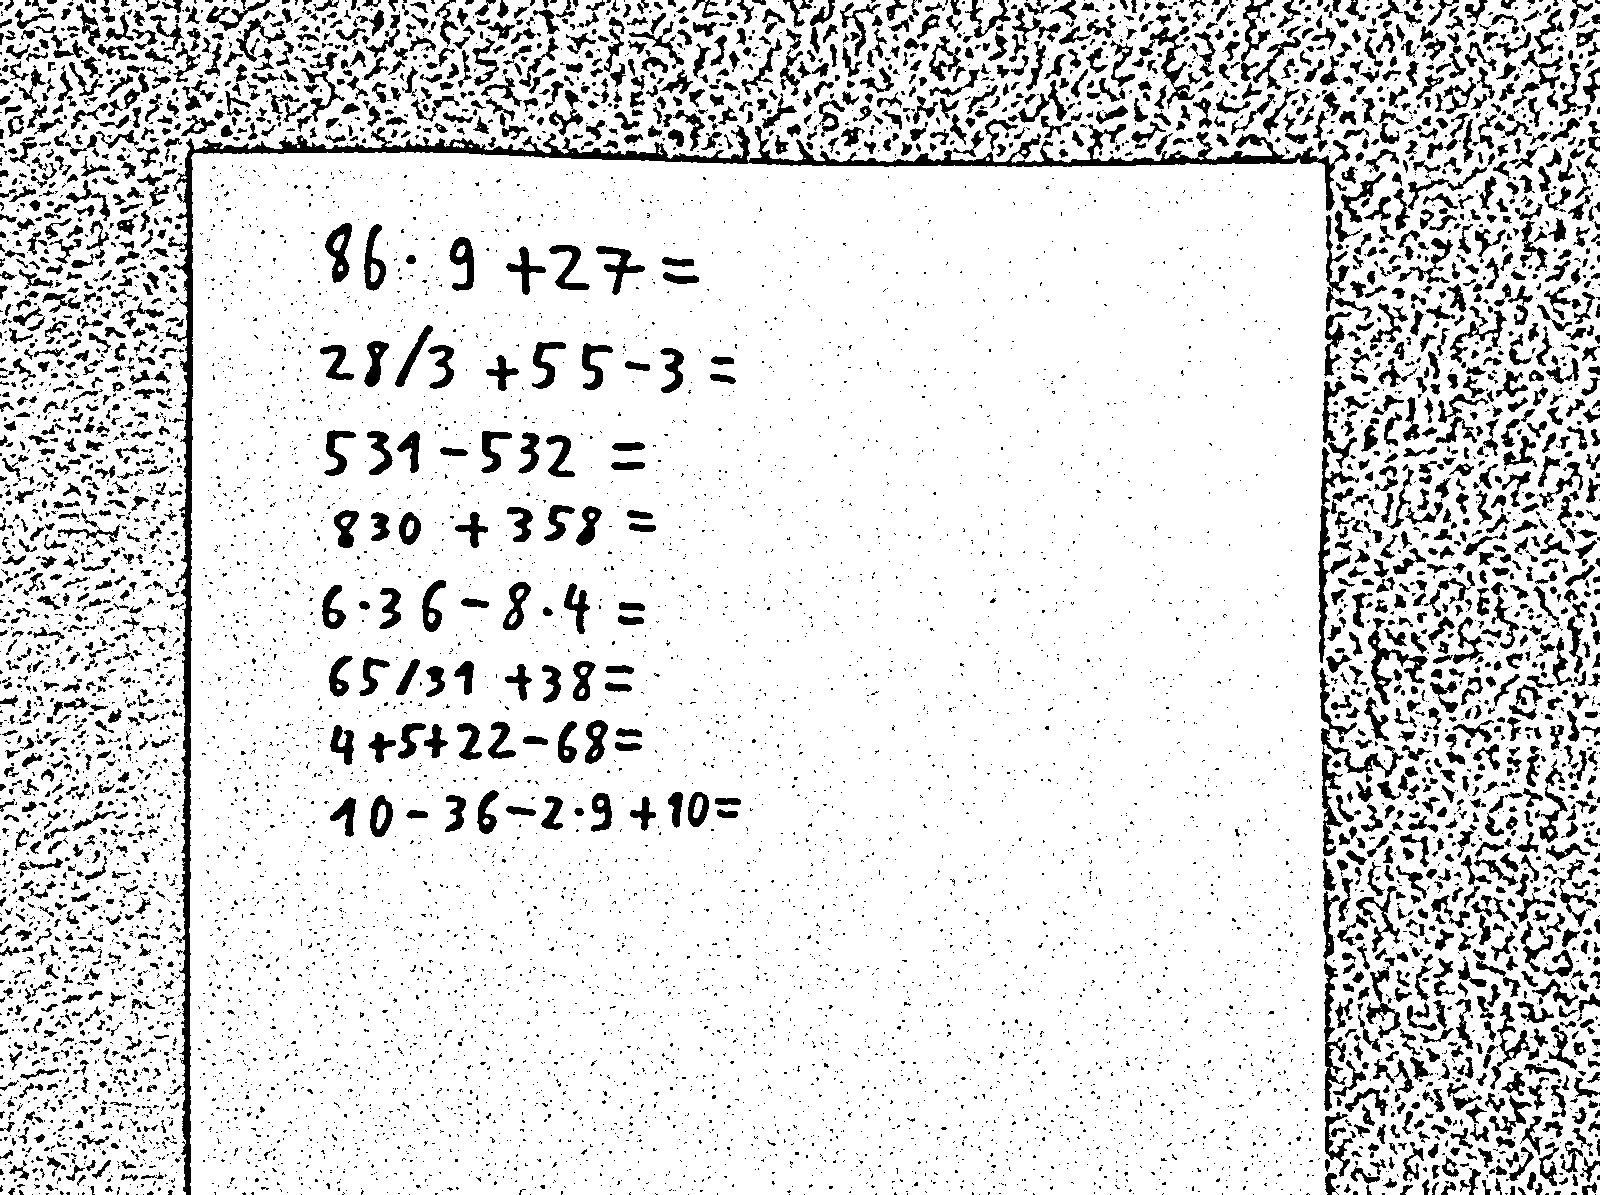
\includegraphics[width=.8\linewidth]{ImagesForReport/AdaptiveGaussianThresholding}
%			\caption{Adaptive Gaussian Thresholding}
%			\label{fig:AGT1}
%		\end{subfigure}
%		
%		\begin{subfigure}{.5\textwidth}
%			\centering
%			\includegraphics[width=.8\linewidth]{ImagesForReport/Dilation}
%			\caption{Dilation}
%			\label{fig:Dilation1}
%		\end{subfigure}\\
%		
%		\caption{Various Steps performed during the Simple Preprocessing Process}
%		\label{fig:SimplePreprocessing}
%	\end{figure}


		The image our program receives as input is likely not easily analyzed as is.
		We therefore pre-process the image with a few select operations before continuing with our algorithm.
		It should be noted here that there is a great variety of different algorithms that work well.
		The algorithm we will be presenting here is the one we found to work well for our purpose.\\
		It operates in five steps (see fig: \ref{fig:SimplePreprocessing}):
		\begin{itemize}
			\item Grayscaling: At first, we grayscale our image.
			Here, we reduce the BGR (blue, green, red) image into one with a single dimension per pixel.
			This is useful, because it simplifies the image and allows us to more easily analyse it.
			\item Gaussian Blur: Here, we apply a Gaussian blur kernel on the image to smooth it out. This reduces the noise.
			\item Morphological Opening: We apply a filter that removes a specific type of noise: small dots. This is done by applying an erosion followed by a dilation filter. %??? is this the right filter
			\item Adaptive Gaussian Threshold: We add a filter that applies a threshold. 
			Any pixel below this threshold gets set to 0 and any pixel above it gets set to 255. %??? check
			This threshold differentiates the symbols from the background.
			We will later explain in more detail how this filter works. %??? !!! Do it
			\item Dilation: After the previous steps, it is possible that some of the symbols have decomposed into several parts.
			This allows for easier contour detection.
			However, this makes the contour more difficult for the classifier to recognise, which is why this step will be undone later. %??? Errosion is Dilation correct?
%			(Because our image is inverted, the code uses an erosion function.) %??? fix
			Therefore, it is useful at this point to thicken the contours.
		\end{itemize}
	%	\begin{lstlisting}
	%def preprocess(self, img):
	%	preprocessed = self.convert_gray(img)
	%	preprocessed = self.gaussian_blur(preprocessed)
	%	preprocessed = self.morph_open(preprocessed)
	%	preprocessed = self.binarize(preprocessed)
	%	preprocessed = self.erode(preprocessed)
	%	return preprocessed
	%	\end{lstlisting}
			
	
	\subsubsection{Border Removal}%??? !!! Add before vs after Images, after Preprocessing is complete
		\small{Author: Timothy Jay Herbst} \newline \newline
		After these pre-processing steps, we have a fairly good image.
		However, very often the shape of background objects register as contours.
		THis section explains how to remove the contours of background objects.
		For this, we make use of a simple observation: symbols tend to be separate from other contours, while background contours tend to be flaky and can be roughly traced to the border of an image, see fig .%???
		Using this knowledge we can create a mask, which removes the background contours.\\
		We determine the mask in the following steps:
		\begin{itemize}
			\item Simple Preprocessing: At first we need to simplify the image. We use a similar algorithm as used in the section "Simple Preprocessing" for this.
			\item Adding a Border: For the next step we add a black border to the image. Our aim is to remove all contours which connect with this border.
			\item Strong Dilation: We now repeatedly dilate the image. Our goal here is to connect all contours which are close to each other.
			Unfortunately this makes our contours unreadable.
			This is not a problem since in this step we simply want to determine the contours we want to keep.
			\item Floodfill Border: We then floodfill the border.
			This removes any contour which connects to the border. 
			\item Remove Border: Since we changed the image size by adding a border, we now have to remove it.
		\end{itemize}
		In this manner we determine the mask.
		Our resulting image is determined, by having all pixels white, except those, that are black both in the mask and in the simple preprocessing.
		This removes background contours, without making our image unreadable.
	\begin{figure*}[htp]
		\centering
		\subfigure[Original Frame]{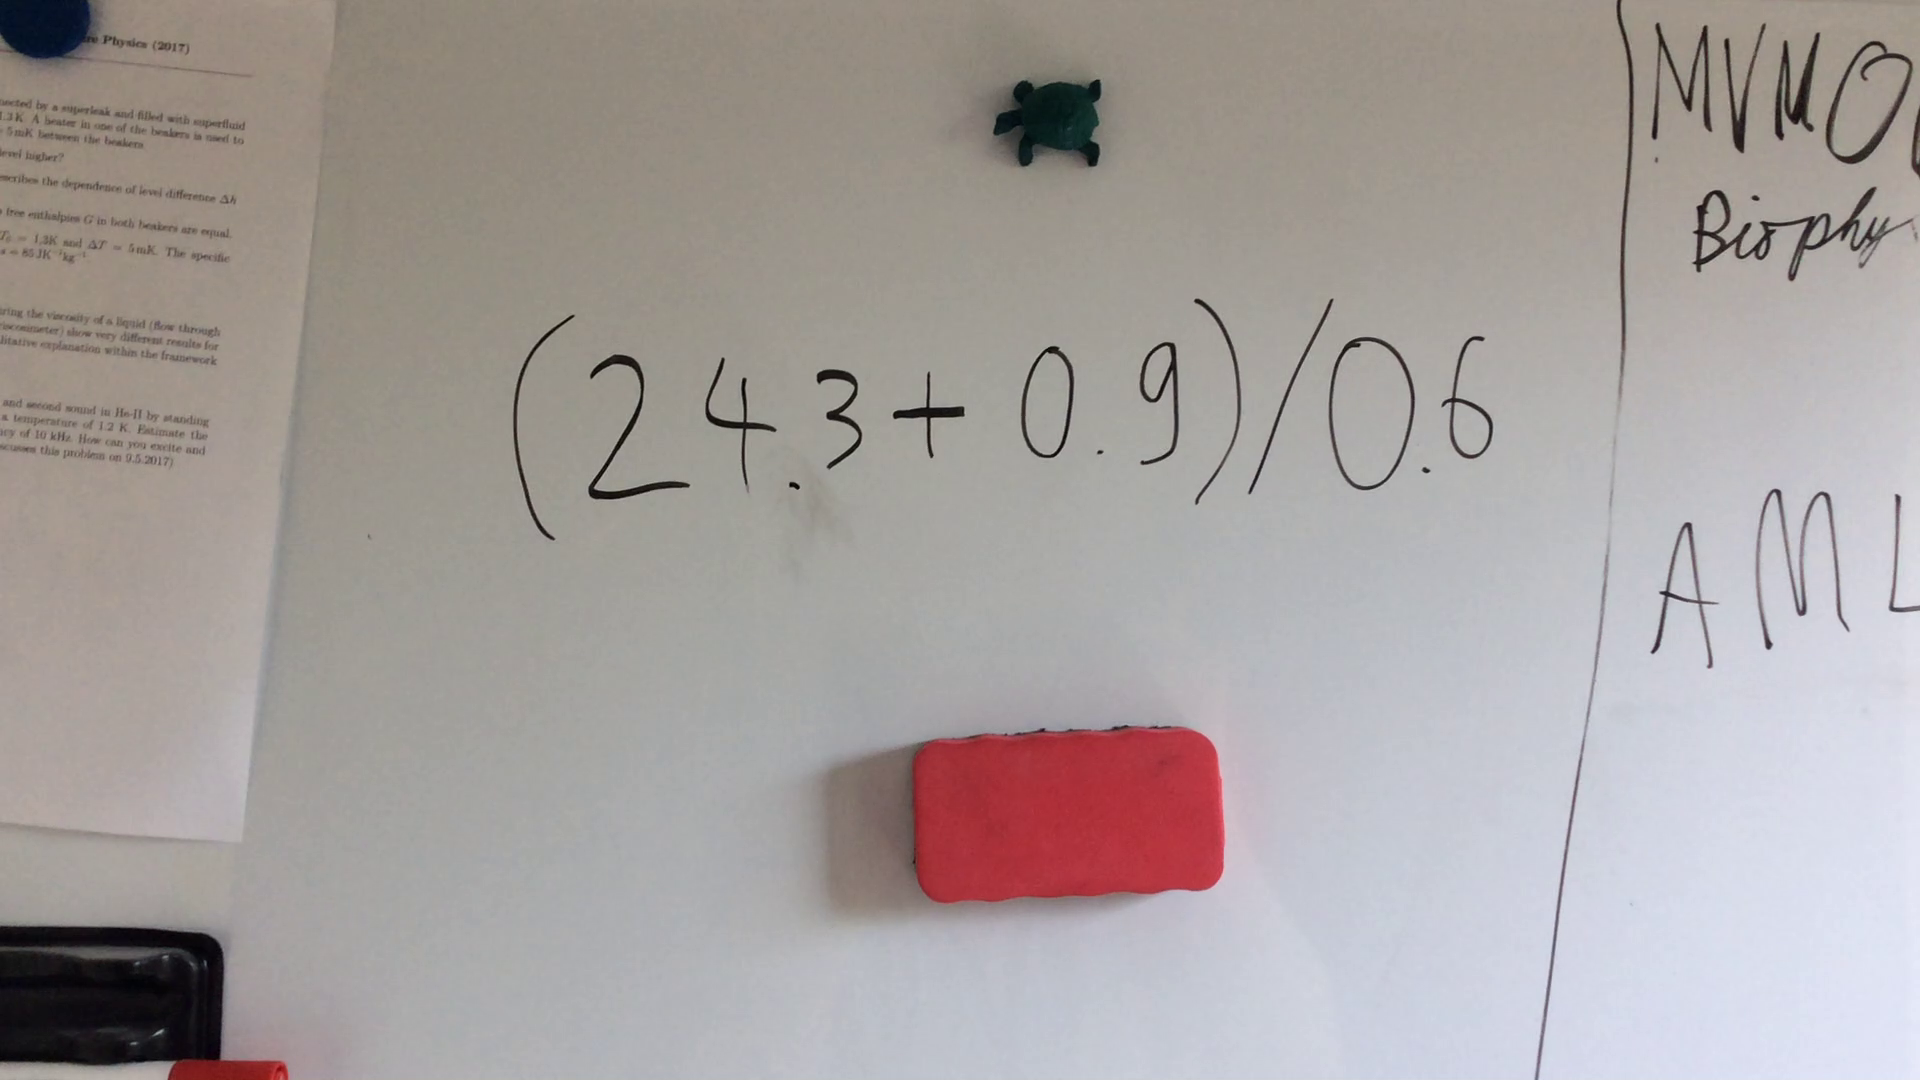
\includegraphics[width=.45\linewidth]{ImagesForReport/Frame2}}\quad
		\subfigure[After Simple Preprocessing]{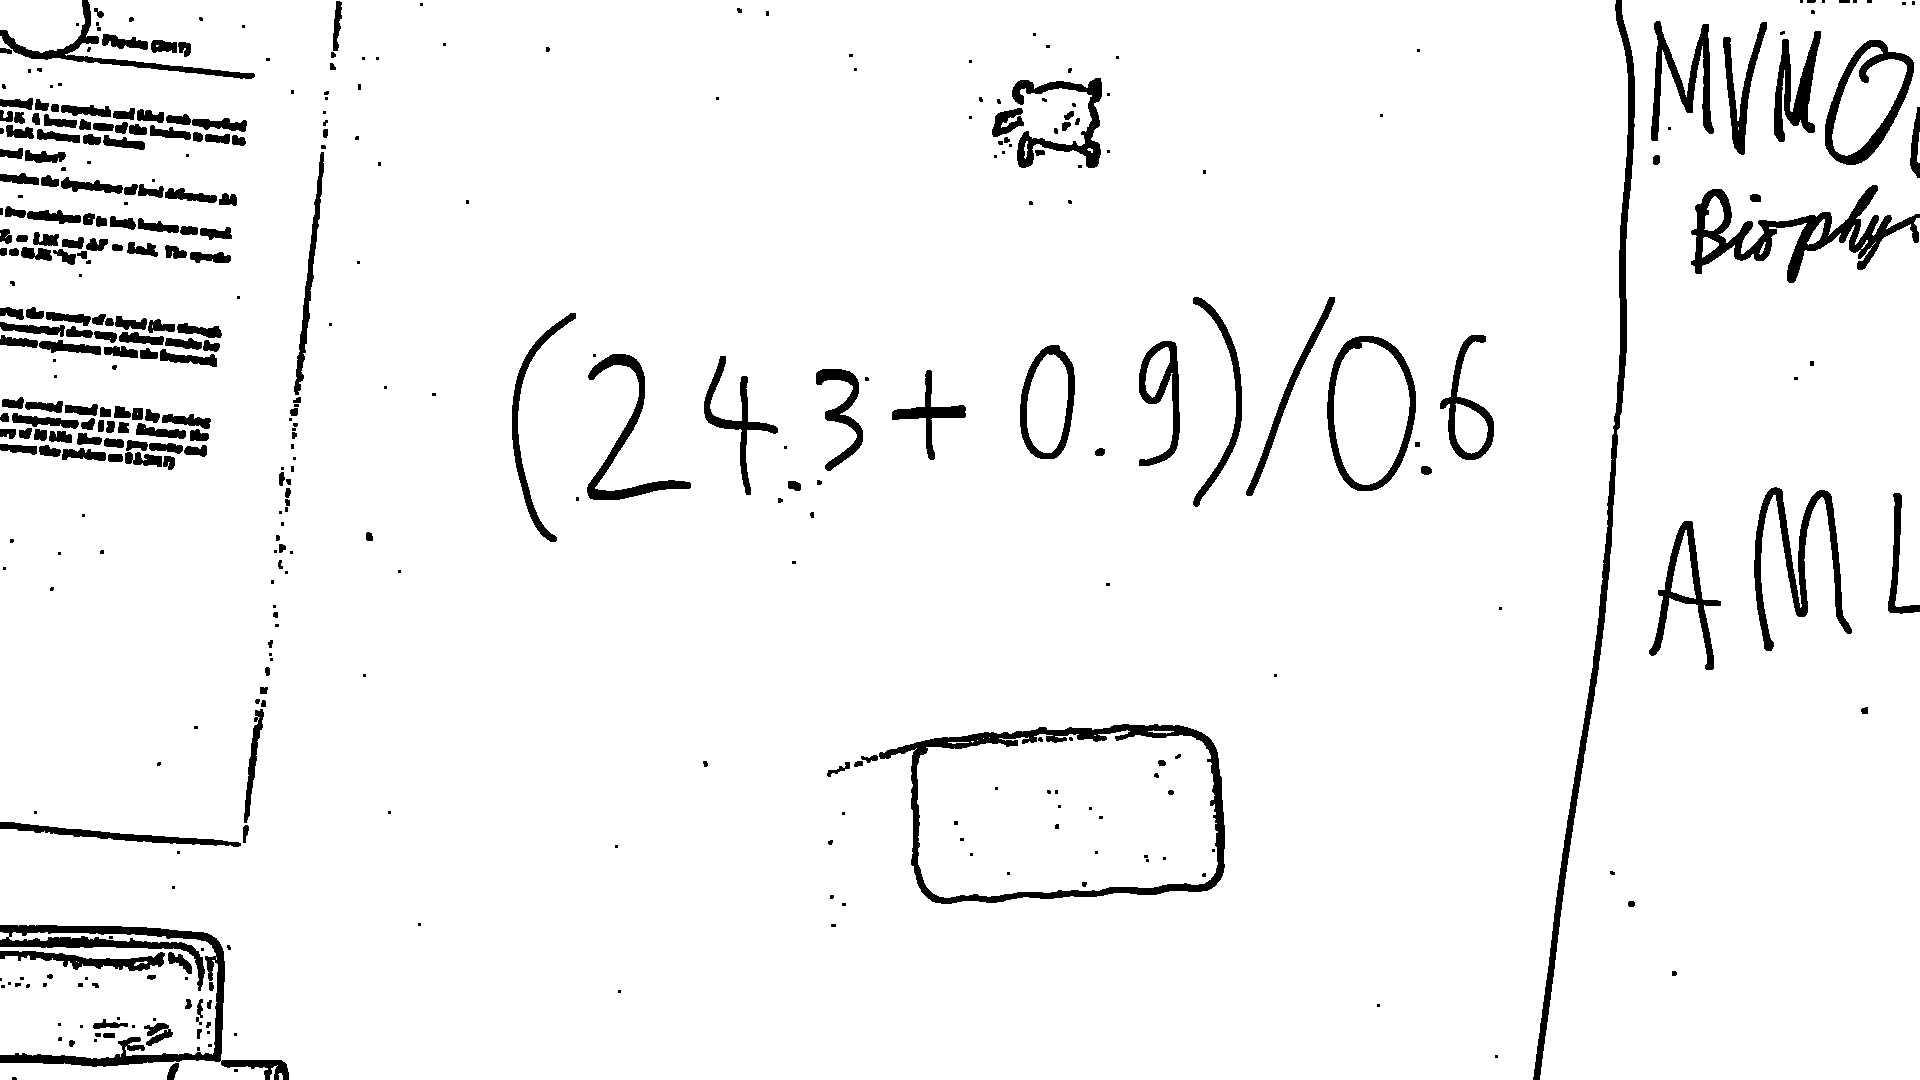
\includegraphics[width=.45\linewidth]{ImagesForReport/PostPreprocessed2}}
		
		\subfigure[Border Removal Mask (Black pixels will not be removed)]{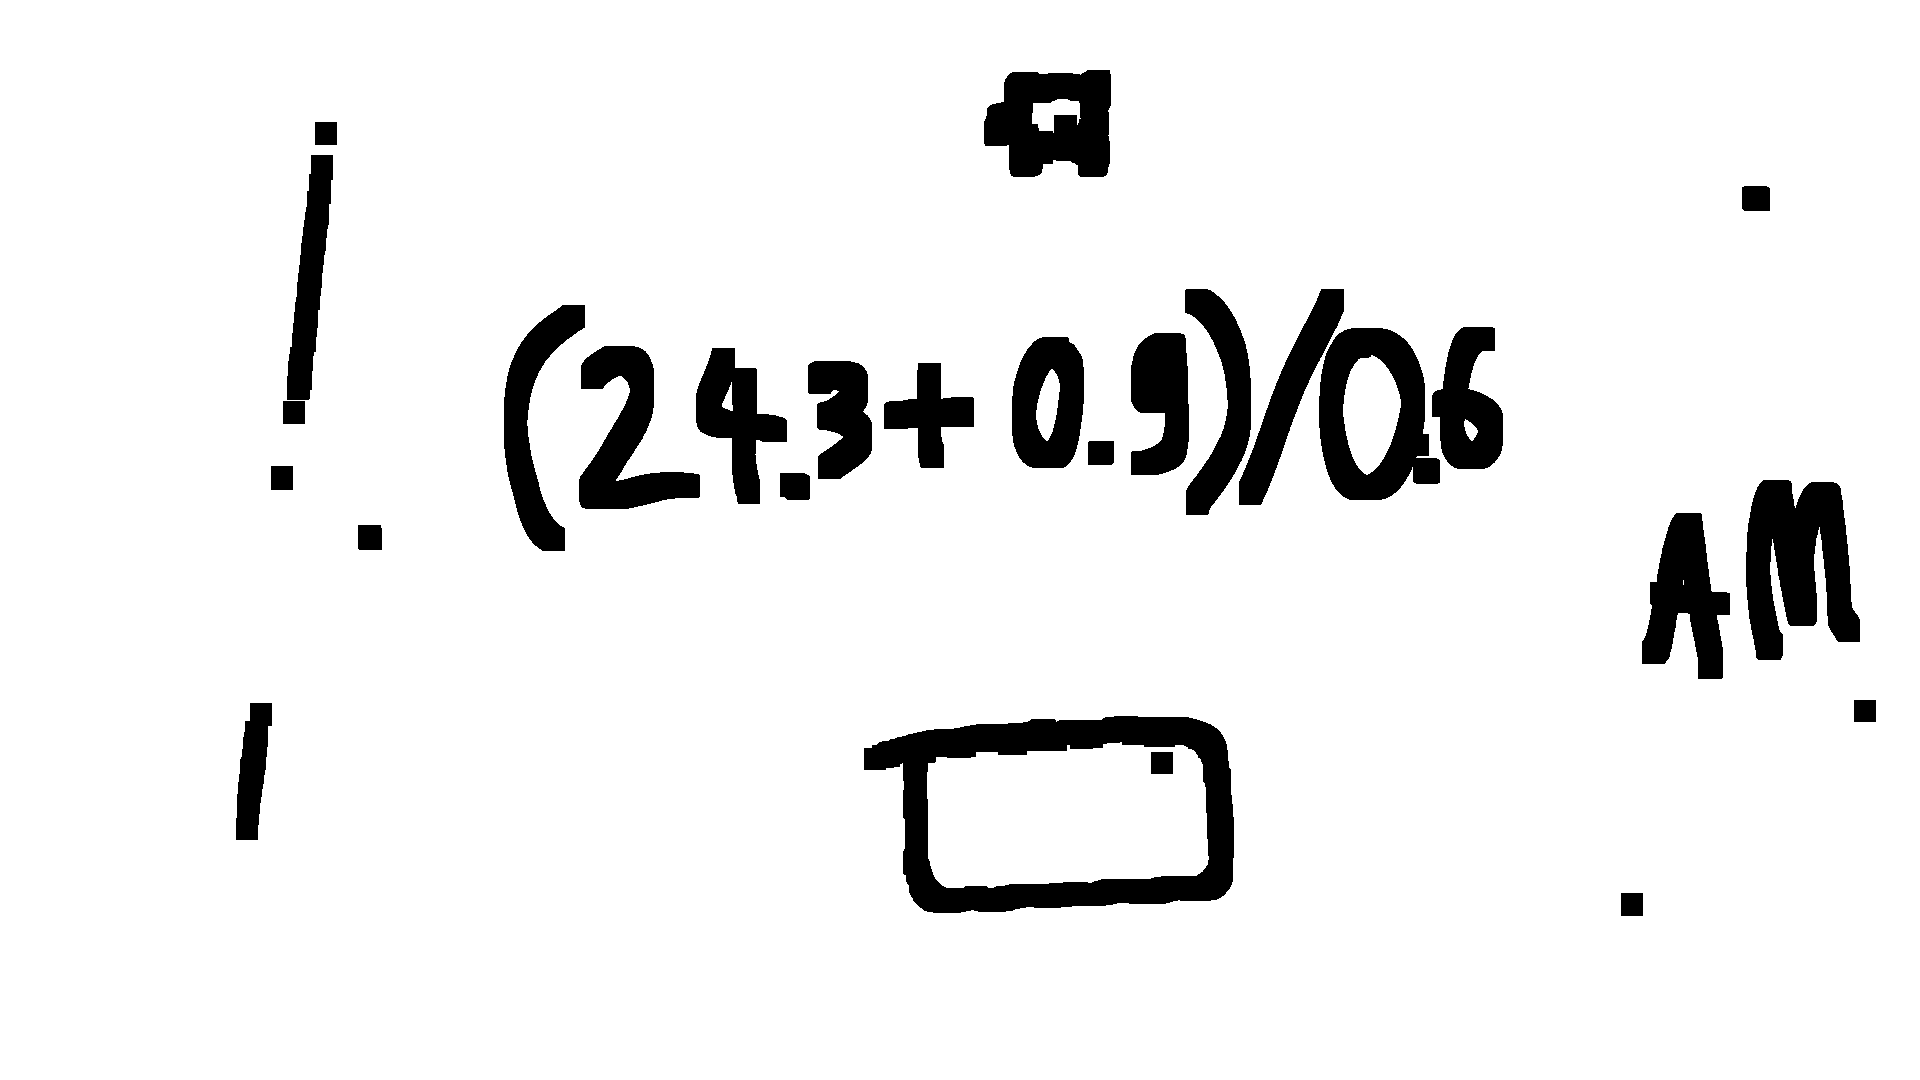
\includegraphics[width=.45\linewidth]{ImagesForReport/backgroundMask2}}\quad
		\subfigure[Resulting Image]{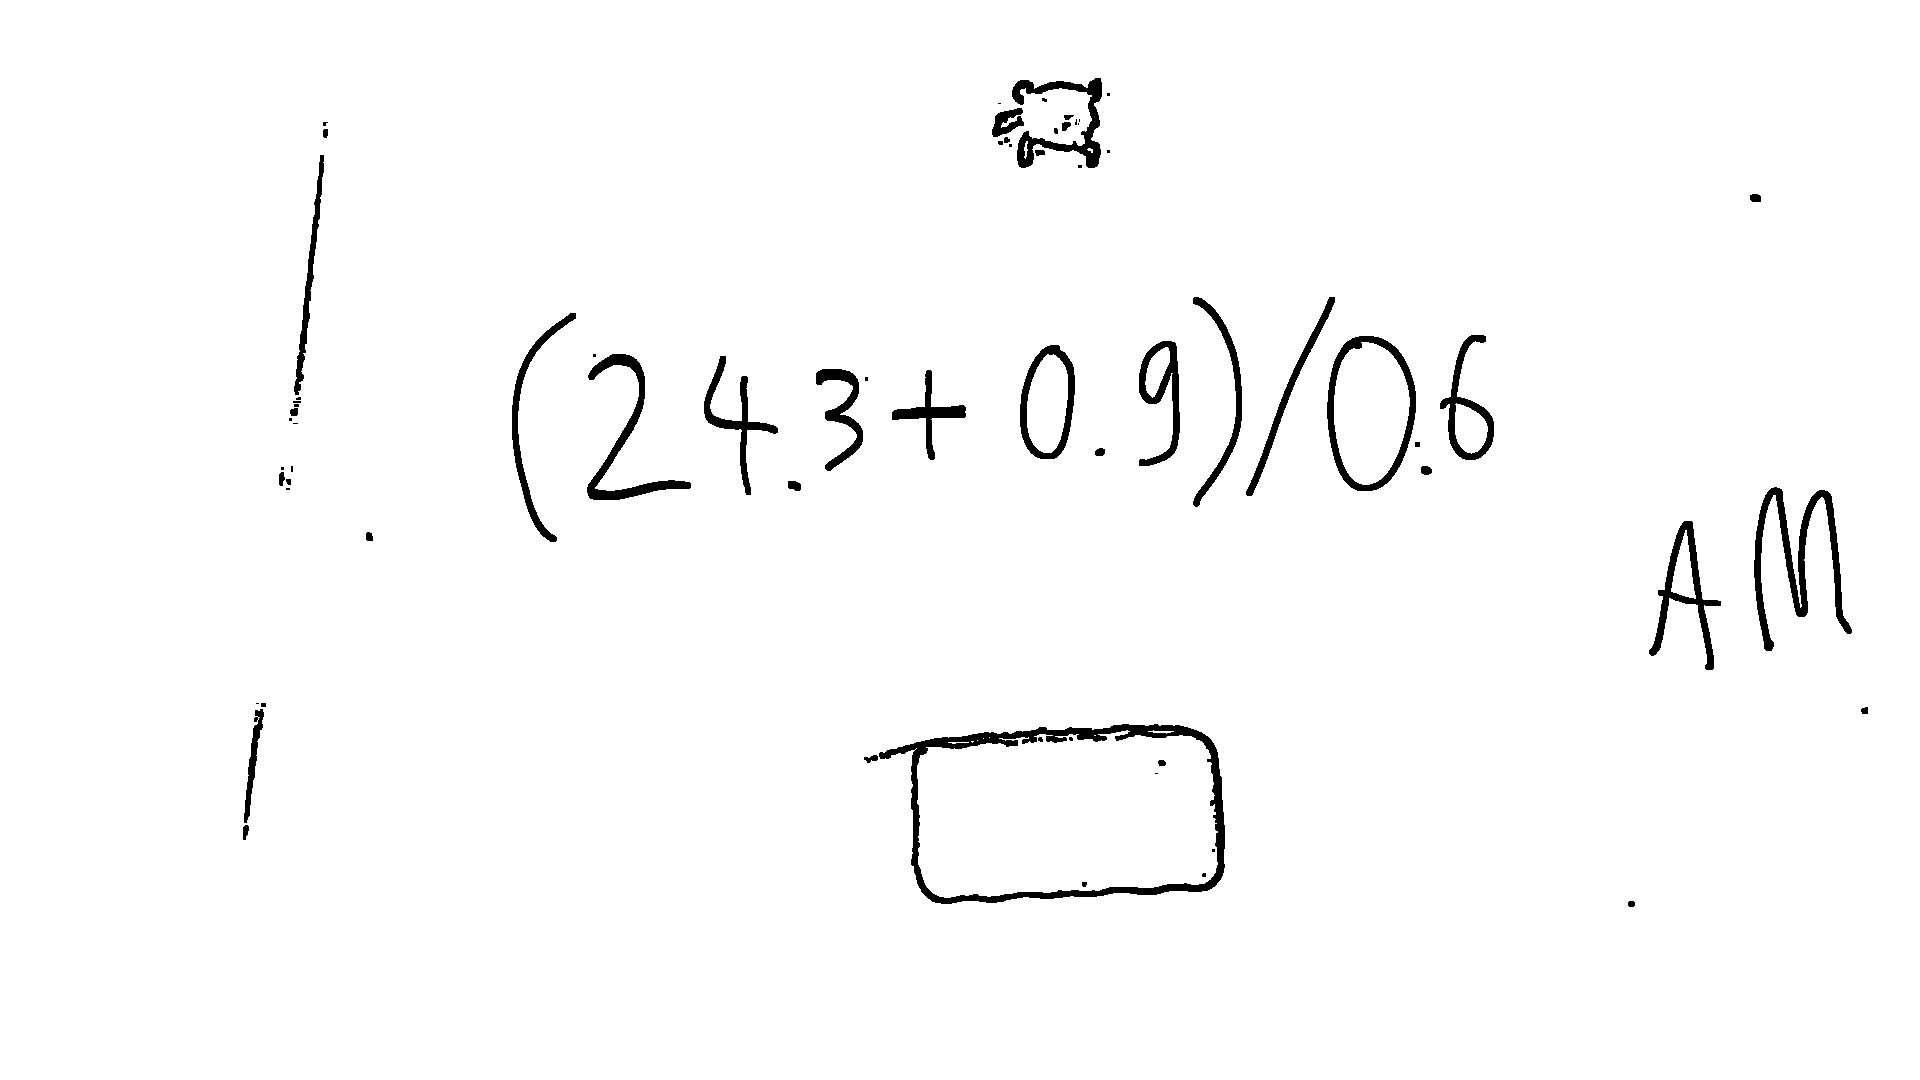
\includegraphics[width=.45\linewidth]{ImagesForReport/BackgroundRemoved2}}
		
		\caption{Performance of the Border Removal Mask.}
		\label{fig:BorderRemoval}
		%??? Make captions in center
	\end{figure*}
	
	\subsubsection{Reflection Removal}
	\small{Author: Timothy Jay Herbst} \newline \newline
	Bright light sources may reflect off the surface on which the equation is written.
	This occurs especially often when using a white board, but also on paper (see fig. \ref{fig:BrightnessRemoval}).
	Unfortunately, the adaptive threshold function cannot differentiate between the writing and the bright reflections.
	Fortunately, the reflected light sources all have a commontrait:
	They are significantly brighter than the average image.
	It is therefore possible to create a fairly simple mask which simply removes all pixels which are significantly brighter than the average pixel of the image.
	After applying this mask, the image no longer contains contours caused by reflected light sources.%??? significantly
	
	\begin{figure*}[htp]
		\centering
		\subfigure[Original Frame]{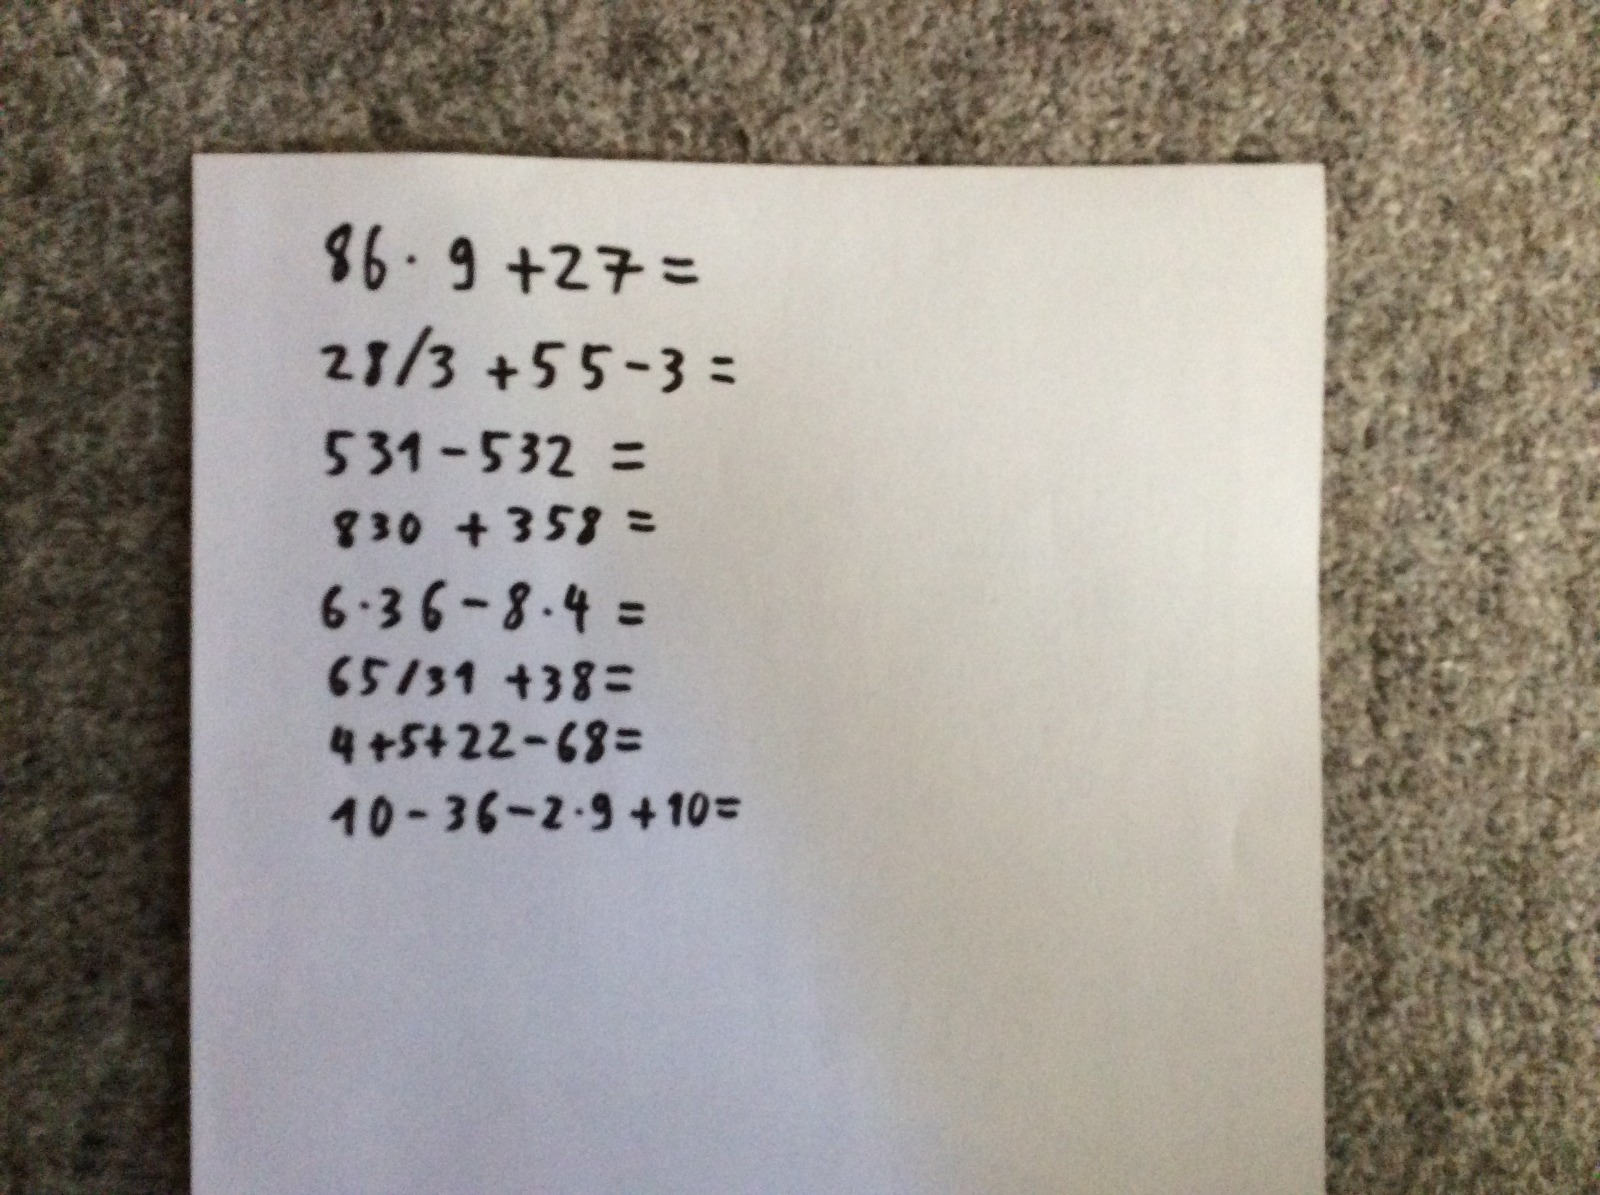
\includegraphics[width=.45\linewidth]{ImagesForReport/Frame}}\quad
		\subfigure[After Simple Preprocessing and Background Removal]{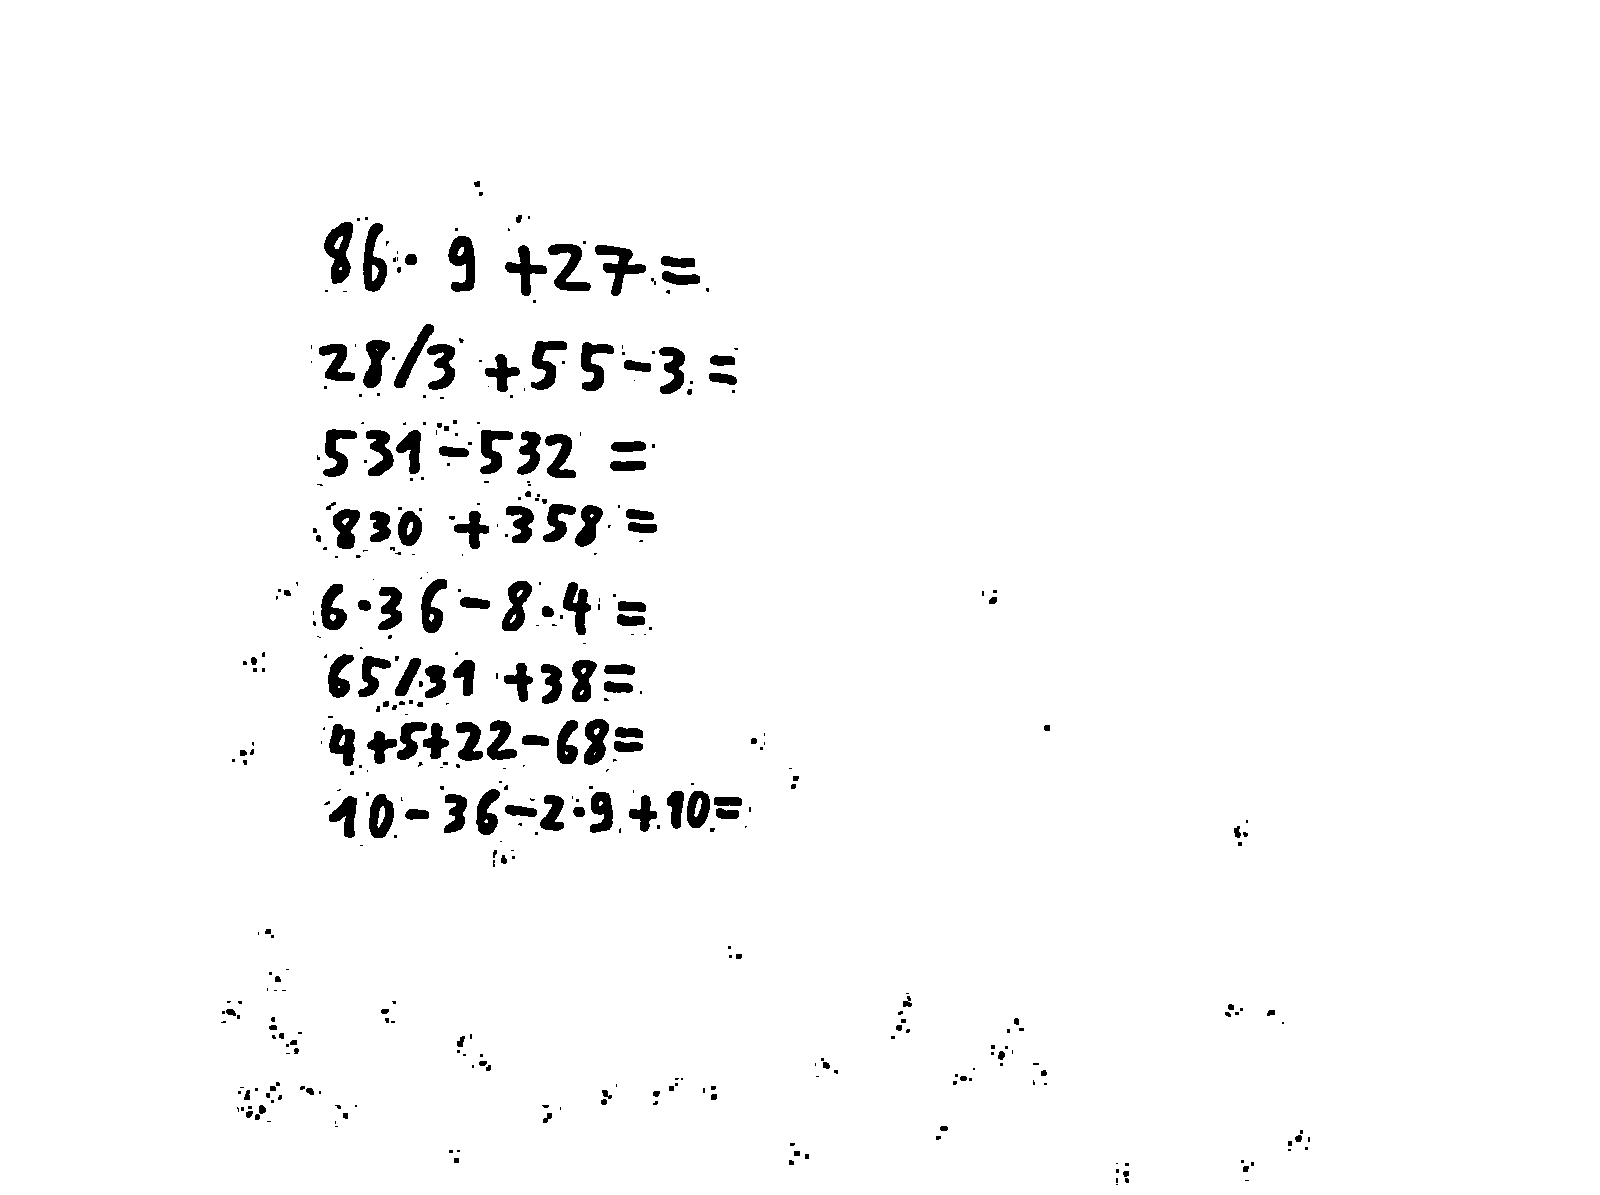
\includegraphics[width=.45\linewidth]{ImagesForReport/BackgroundRemoved}}
		
		\subfigure[Reflection Removal Mask (Black pixels will not be removed)]{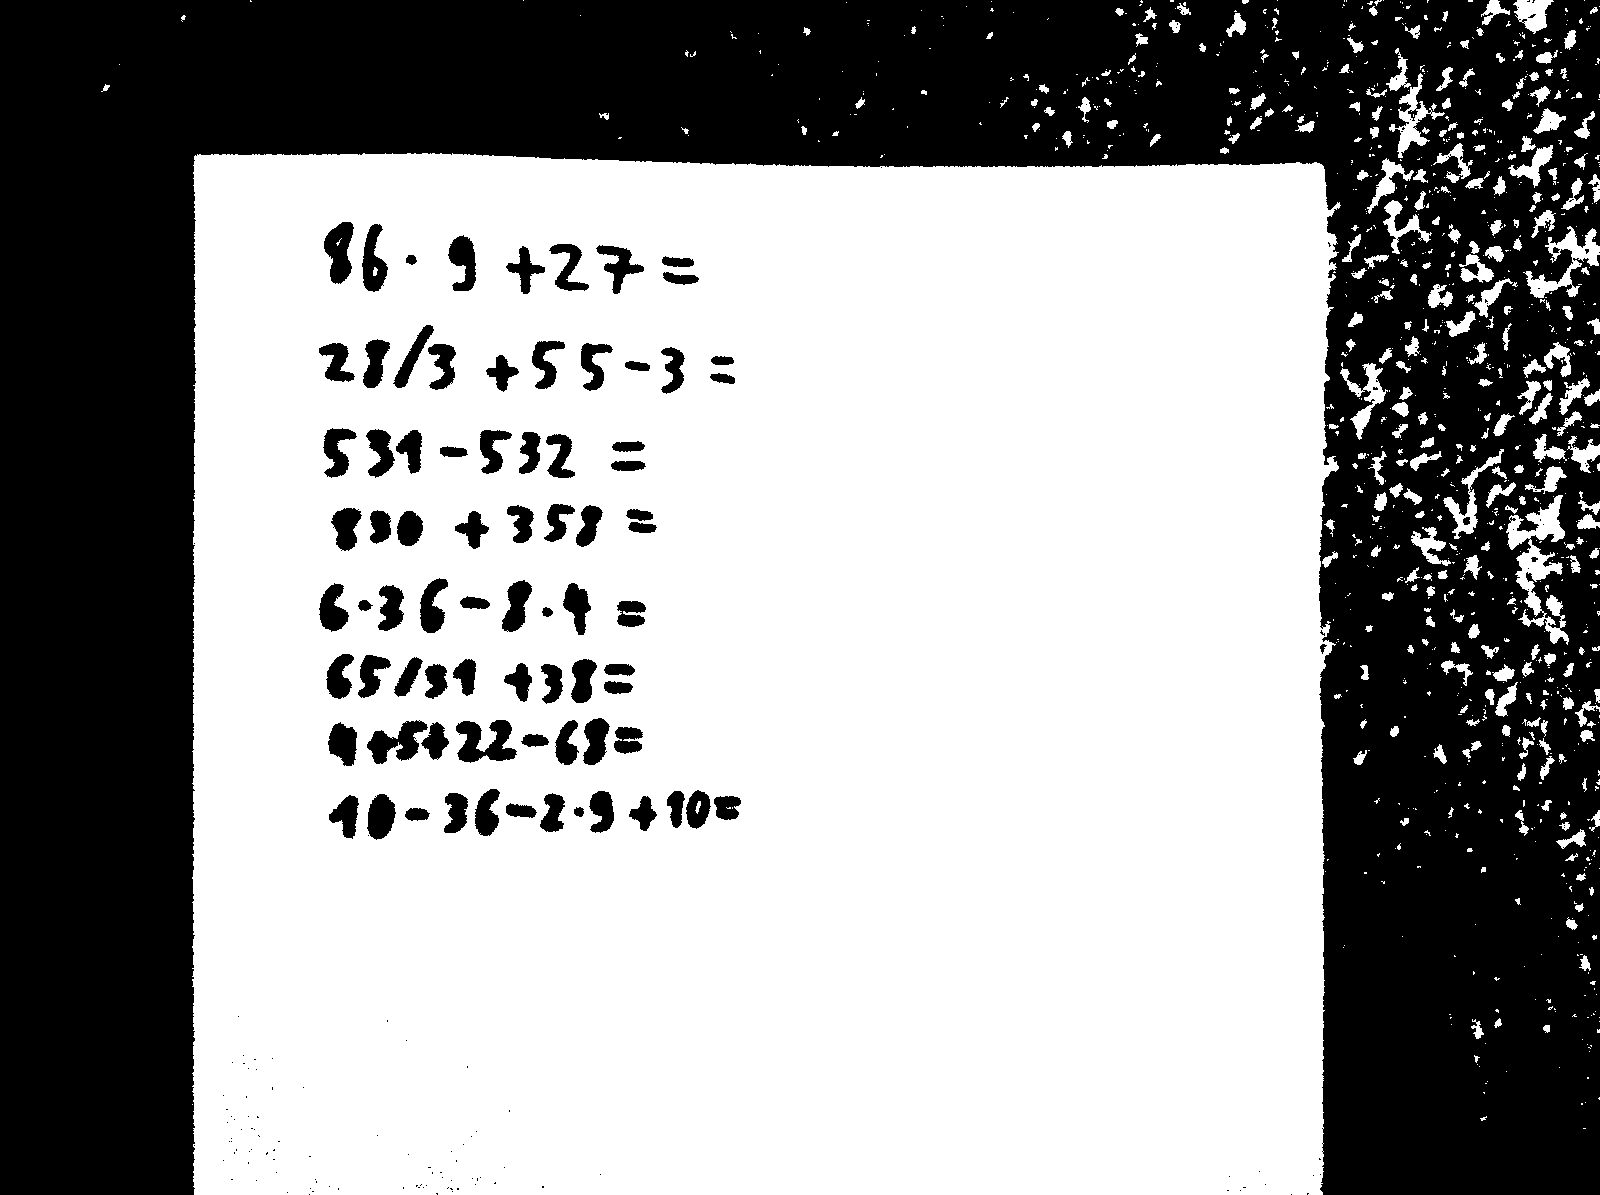
\includegraphics[width=.45\linewidth]{ImagesForReport/BrightnessMask}}\quad
		\subfigure[Resulting Image]{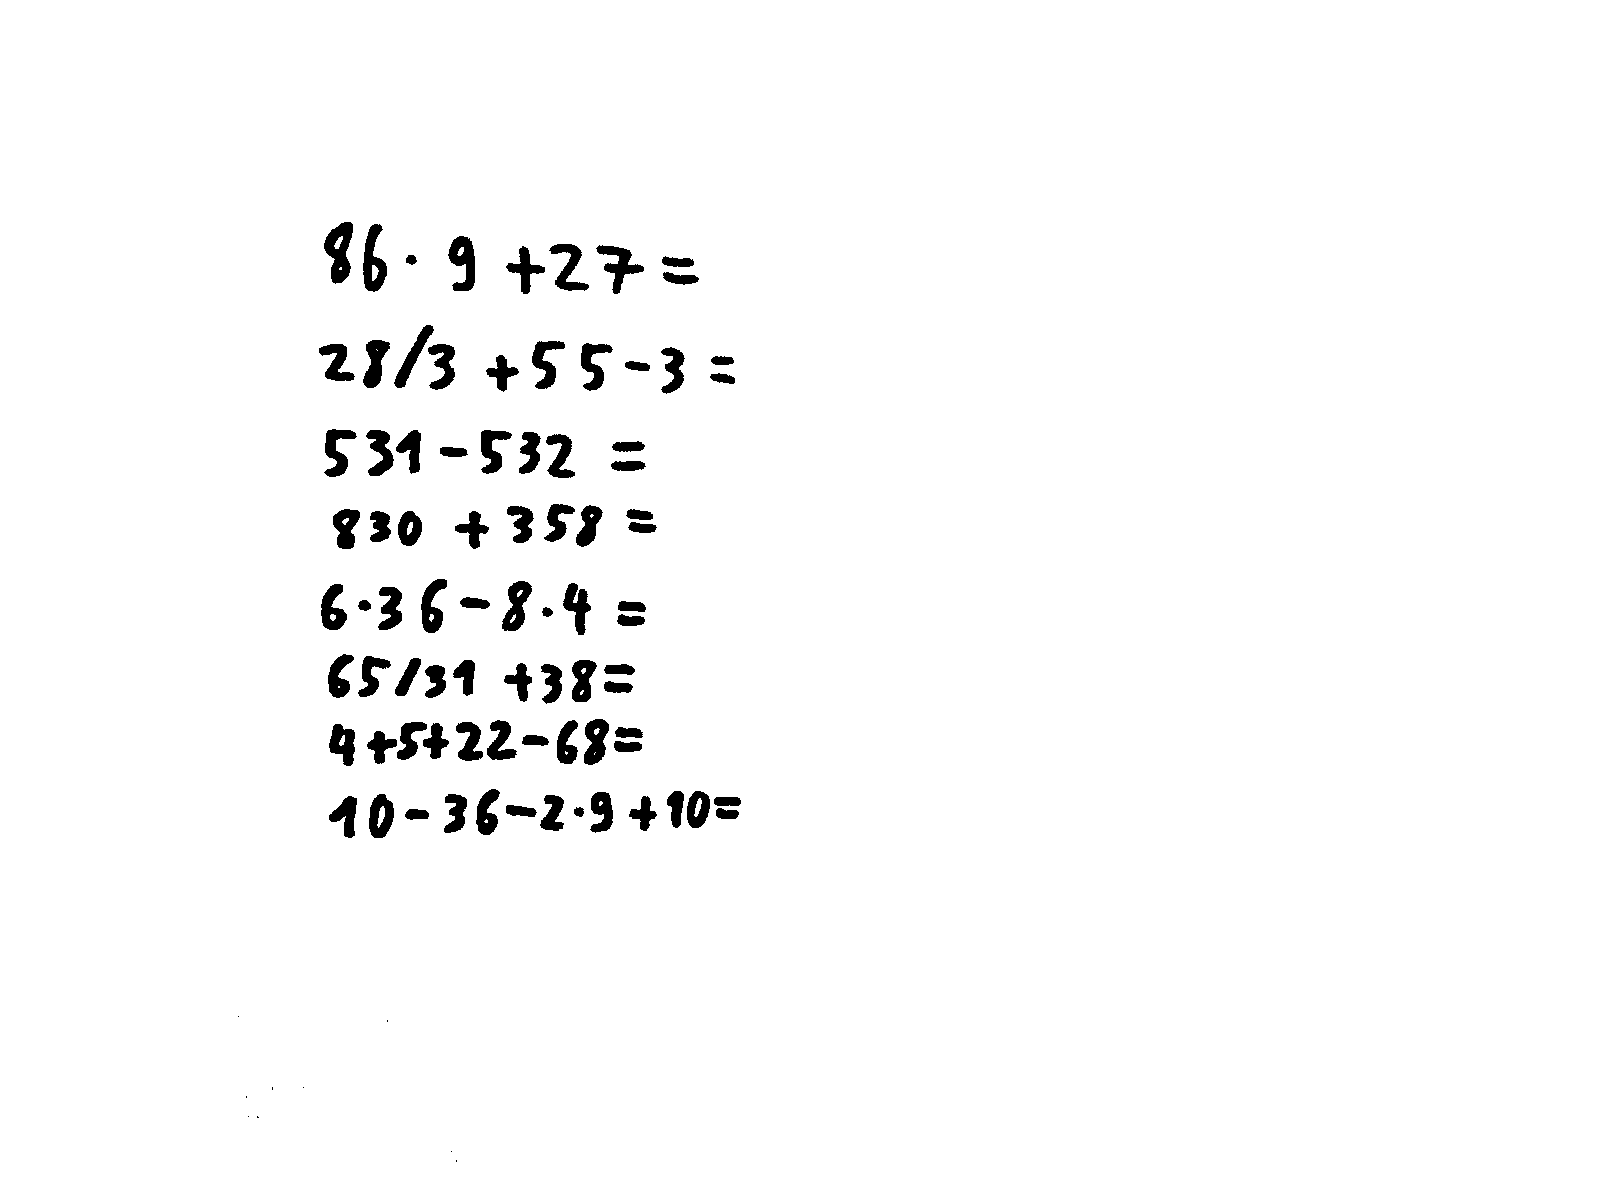
\includegraphics[width=.45\linewidth]{ImagesForReport/BackgroundFiltered}}
		
		\caption{Performance of the Reflection Removal Mask.}
		\label{fig:BrightnessRemoval}
		%??? Make captions in center
	\end{figure*}
	
	
	
	
	\subsection{Segmentation}
		\small{Author: Duc Anh Phi} \newline \newline
	In the segmentation step, we extract written characters from the image.
	These extracted pixels are then further evaluated - they make up the building blocks of our program.
	In the following and sections to come, we are going to detect, group, order and classify these segments, in order to
	reproduce and finally solve the written equations.
	
	\subsubsection{Contour Detection}
	\small{Author: Duc Anh Phi} \newline \newline
	After the preprocessing is done, we can deploy an algorithm to detect contours from the image.
	In simple terms, a contour is the boundary of an object in the image.
	The library\texttt{OpenCV} defines a contour as a ``curve joining all the continuous points (along the boundary), having the same color or intensity".
	These contours are essential for later shape analysis, object detection and recognition.
	
	The underlying algorithm we used for contour detection is from the paper Suzuki et. al. (1985).
	This paper presents a border following technique for binary images. "It derives a sequence of the coordinates [...]
	from the border between a connected component of 1-pixels (1-component) and a connected component of 0-pixels (background or hole)."
	Not only does the algorithm reliably detect contours, but also it gives us hierarchical information about them.
	
	This will be important for making sense of nested (contours completely inside of other contours) contours later.
	
	\subsubsection{Removing Small Contours}
	\small{Author: Duc Anh Phi} \newline \newline
	Not all segmented contours represent handwritten signs.
	Some are noise which passed the preprocessing. Usually, this noise is rather small, e.g. points or thin lines.
	With the assumption that handwritten signs have approximately equal line thickness, we can confidently remove all contours which have a significantly smaller line thickness.
	For this to work well, we have to find a good threshold line thickness.
	Computing the average line thickness is costly and might be inaccurate for images with lots of small noise.
	To make sure not to include the line thickness of noise, contours of median size are selected. Then, we compute the line thickness for each of these selected contours.
	The median out of these computed values is our threshold line thickness.
	
	\paragraph{Compute Line Thickness}
	\small{(Author: Duc Anh Phi)}\\
	The algorithm for computing the line thickness of a contour was taken from \url{https://cs.stackexchange.com/questions/59475/width-of-a-string-line-in-an-image}
	\begin{enumerate}
		\item We start with a binary image (see fig. \ref{fig:linethickness}), with pixel values either zero (black) or 255 (white).
		\item Summing up the image gives us the sum of all white pixels, as black pixel are zero. In other words, the sum gives us the area of the whole white line (in pixel times 255).
		\item After skeletonizing the image, the white line becomes one pixel thick (see fig. \ref{fig:linethickness}). The resulting skeleton is a 1-pixel-thin approximation of the original image.\\
		Summing up the skeleton gives us the approximate length of the line.
		\begin{align}
		Area = Sum/255
		\end{align}
		\item With the line area and length, we calculate its thickness as:
		\begin{align}
		Thickness = Area / Length
		\end{align}
	\end{enumerate}

	\begin{figure*}[h!]
		\centering
		\subfigure[Original Contour]{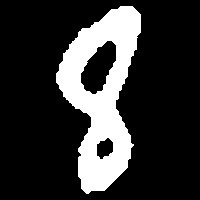
\includegraphics[width=.45\linewidth]{ImagesForReport/orig.jpg}}\quad
		\subfigure[After Skeletonizing]{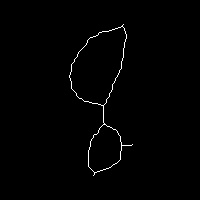
\includegraphics[width=.45\linewidth]{ImagesForReport/skeleton.jpg}}
		
		\caption{Computing the Line Thickness}
		\label{fig:linethickness}
	%??? Make captions in center
	\end{figure*}
	
	\subsubsection{Group Contours}
	\small{Author: Duc Anh Phi} \newline \newline
	Some contours belong together to form a mathematical symbol or structure. In the following, we replace the individual contours with their grouped versions.
	
	\paragraph{Handling Nested Contours}
	For example, a handwritten '8' usually consists of 3 contours: The outer frame and the inner two holes, which are detected as separate contours.
	To not confuse these holes as distinct math symbols, we group them together in a single, custom contour object.
	A contour object has the parent or outermost contour stored in its “contour” property.
	The contours representing holes are stored in the “holes” property.
	
	\paragraph{Fractions}
	Fractions are problematic, as they have an inherent order to them – especially nested fractions.
	This order must be taken into account. Additionally, fractions have multiple (at least 2) expressions stacked vertically, which may span several lines.
	This can cause problems, when evaluating multiple lines of equations, because the numerator or denominator may be accidentally assigned to the wrong line.
	The solution to these problems is to simplify fractions to single contours (their bounding boxes), while still preserving positional information about each grouped element.\\
	Initially, we have to find the fractions. How we find fraction bars is shown in \ref{fractionbar}. After sorting the fraction bars (ascending) by their width we apply the following algorithm to each bar iteratively, starting with the smallest one:
	\begin{itemize}
		\item extract contours above and below the fraction bar (inside the acceptance area) and create a custom fraction object, which references them in the “numerator” or “denominator” property. The acceptance area is inferred from the bar width.
		\item sort each contour in the “numerator” or “denominator” property by their x-coordinates – in this way, we ensure a correct order
		\item create a bounding box around the whole fraction
		\item create a contour object based on the bounding box and the Fraction object
	\end{itemize}

	\paragraph{Equal Sign}
	A written “=” sign consists of two vertically stacked horizontal bars. We group both contours in a single contour object. How we find equal bars is shown in \ref{equalbars}. Once an equal bar is found, we create a bounding box around itself and its counter part.
	A new contour object is created with the bounding box as its "contour" property.
	
	
	\subsection{Line Assignment and Ordering}
	\small{Author: Duc Anh Phi} \newline \newline
	At this stage, we have a list of (grouped) contour objects. We now face the problem of bringing them into correct mathematical order, based on their position in the image.
	This task seems trivial for one equation: simply sort the contours by their x-coordinate.
	However, we aim to solve multiple equations, which are each written in a separate new line.
	So, looking at the x-axis is not enough. We have to take the y-axis into account, too.\\* When observing lines of equations, we noticed that all symbols within the same line have a similar y-coordinate value. However, that value will change particularly between lines. With this observation, we developed the following algorithm to separate lines:
	\\
	\begin{enumerate}
		\item Initially, contours are sorted by their y-coordinate. In this way, contours which are in the same horizontal line are closer to each other.
		\item Afterwards, the average y-distance between neighboring contours is calculated:\\
		\begin{align}
		Average Neighbor Y Deviation = 1/N &\sum\limits_{k=2}^{N} \left|y_{k} - y_{k-1}\right|
		\end{align}
		We use this y-deviation as a threshold value to determine whether a new line has started.
		\item In the sorted list of contours, each contour (except for the first) is compared to its predecessor for calculating the y-coordinate deviation between them. If the calculated value is within the y-deviation threshold, both belong to the same line. However, if the calculated value is greater than the reference y-deviation, a new line starts with the current contour.
		\item After extracting lines, each contour in a line is then sorted by their x-coordinate.
	\end{enumerate}
	
	For the Line Assignment we have developed several algorithms. In the following, we discuss the most interesting, the ones able to tackle a particular problem and the most efficient ones.
	
	\subsubsection{Determining the Direction of Writing}
	\small{Author: Timothy Jay Herbst} \newline \newline
	When writing an equation, most people tend to write roughly along an "invisible line".
	Therefore, when taking an image of said equation, we can expect it to adhere roughly to the line.
	We can use this to determine the order of the symbols.\\
	There are however, two issues with this:\\
	Firstly, unlike a computer a human will not precisely write their symbols in a line.
	Oftentimes a symbol will be significantly above or below said line.
	It gets even worse, if we take a look at exponents, division bars and similar.\\
	Secondly, the "invisible line" may not be along the horizontal of an image.
	This may be because of sloppiness of the writer, or because the image was taken at an angle.\\
	Because of this, it is very useful to be able to determine the direction of such an "invisible line".
	In the following we will be discussing a method how to determine this line.
	It should be noted at this point however, that in most images we took this "invisible line" deviates by less than $10^\circ$.
	All of the following algorithms are capable of dealing with such small deviations.\\
	
	
	
	%\subsection{A Naive Approach}
	%This section aims not to introduce a particular algorithm, but to illustrate some of the problems such an algorithm must face.
	
	%A naive approach to assigning lines, may be to assume two symbols are within the same line, if they are close to each other.\\
	%This could be implemented, by determining a radius of acceptance $R$.
	
	\subsubsection{Assigning Lines to Proposed Line Positions}
	\small{Author: Timothy Jay Herbst} \newline \newline
	Our aim is to accurately order the contours into lines.
	A possible method for doing this is by proposing the position of lines.
	Then we check for each proposed line, whether or not a given contour is a good fit (if it is within a certain radius of the line).\\
	For this procedure we at first have to find a rough estimate of the diameter of a line.
	This can be done in a variety of different ways.
	The best method we found at first determines the extension (radius of minimal enclosing circle) of every single found contour.
	Of these, the biggest radius that isn't part of a fraction is then chosen to be the presumed line radius.\\
	To find the ideal line position, we propose a great variety of possible lines.
	In practice we choose a line every $0.4 \cdot \mathrm{line radius}$.
	For every one of these lines, the appropriate contours are assigned.
	Because we choose a lot of different lines, it is very likely that contours are present in multiple lines.
	We can find the best lines, by removing all lines, that have a neighbouring lines, which contain more symbols.
	The longest lines correspond to the written lines.\\
	Afterwards, all lines with less than 3 symbols in them are removed.
	This can be done with confidence, because even the smallest equation (e.g. "1+1") has at least 3 symbols.\\
	
	While there are some obvious flaws with this method, it works surprisingly and consistently well.
	It performs especially well, when equations are written along lines with large spaces between symbols.
	Compared to other methods it can maintain the position of a line and doesn't wander into other lines.\\
	It does however, have difficulty if there are hazy patches in an image, which cause a large amount of wrong contours close to each other.
	The algorithm will always attempt to place a line around these contours.\\
	Another issue is caused, if the lines are written too close and there is a large contour.
	If this is the case, then the line might be placed in between both lines and use contours from both lines.
	%!!! ??? Add more issues
	%!!! ??? Add images
	
	\subsection{Recognition}
	\small{Author: Timothy Jay Herbst, Fenja Kollasch, Duc Anh Phi} \newline \newline
	\subsubsection{Preclassification}
	\small{Author: Timothy Jay Herbst, Duc Anh Phi} \newline \newline
	Given the size, shape and positional information along with the order in which the symbols are written it is possible to classify certain symbols without the need for a neural network. This is very beneficial for two main reasons. The classification problem becomes easier as there are less classes to differentiate from. Additionally it saves computational time, as less contours have to be passed through the network. As a drawback the rule based classification might be less accurate.\\
	We assume that symbols need to have a simple shape while sill being distinct, in order to be accurately classified by certain local rules.\\
	We came up with these rules based on experimentation.
	
	\paragraph{Identify Bars and Points}
	\small{Author: Duc Anh Phi} \newline \newline
	There are mainly two shapes of interest which are used as a basis for further classification: points and bars. They are significant as many math symbols are based on them, e.g. fraction bars, minus signs, multiply signs, equal signs and commas. After the shape is found, we can distinguish mathematical symbols from their position in relation to other symbols. We defined the following rules:
	
	\subparagraph{Bars}\label{bars}
	\begin{itemize}
		\item The width of its minimum bounding box is more than twice as big as its corresponding height.
		\item It does not contain any nested contours (holes)
		\item The ratio of its contour area to its minimum bounding box area should exceed 0.7. This ratio ensures that the contour is rather "flat". However we add a tolerance for "long" contours, e.g. contours whose ratio of width to height exceeds 4. These long contours do not have to fulfill the "flatness" criterion, to be regarded as bars. This tolerance comes from the observation, that keeping a straight line gets more difficult, as the line increases in length. 
	\end{itemize}

	\subparagraph{Points}
	\begin{itemize}
		\item The ratio of its contour area to its minimum bounding circle area exceeds 0.8. This ratio ensures that the contour is rather "round". However, we add a tolerance for "small" contours, e.g. contours whose length or width is smaller than 3 times the threshold line thickness \ref{fig:linethickness}. These small contours do not have to fulfill the "roundness" criterion, to be regarded as points. Written points are not always round, especially when writing quickly.
	\end{itemize}

	\paragraph{Preclassify bar-shaped Math Symbols}
	\small{Author: Duc Anh Phi} \newline \newline
	In the following we show how bar-shaped symbols are classified.
	\subparagraph{Fraction Bars}\label{fractionbar}
	We distinguish between vertical and horizontal fraction bars.
	Vertical fraction bars are defined as bars with vertical orientation. Analogous, horizontal fraction bars must have a horizontal orientation. Additionally horizontal fraction bars contain contours above and below them, inside a defined acceptance area. This area is inferred from the bar width.
	
	\subparagraph{Minus Sign}
	Minus signs are similar to horizontal fraction bars except they do not contain any contours above or below them (inside a defined acceptance area).

	\subparagraph{Equal Bars}\label{equalbars}
	While a fraction bar will always have symbols above and below it, equal sign bars always appear in pairs. They either have a single contour (their counter part) above or below them, but never both.
	
	\paragraph{Preclassify point-shaped Math Symbols}
	\small{Author: Timothy Jay Herbst} \newline \newline
	A difficulty with detecting handwritten equations is the common usage of points or point-like symbols.
	This makes it nearly impossible to account for all possible interpretations of this.
	Therefore we have focused on the two most common cases:
	The multiplication dot ("$\cdot$") and the comma or dot indicating a partial number (e.g. "$3,14$" or "$3.14$").\\
	Other important times where a dot appears in an equation, which unfortunately we were unable to cover, include points included in letters (e.g. "$i=\sqrt{-1}$"), the time derivative of a variable (e.g. "$\dot{x}=v$") and the dots included in a definition symbol ("$:=$" or "$=:$").\\  % ??? cite https://en.wikipedia.org/wiki/List_of_mathematical_symbols
	As the line has already been ordered, we are able to take a look at the preceding and following contour.
	
	\subparagraph{Comma}
	If the distance between the contour's center to the lower end of the preceding contour is shorter than the distance between the centers of both, then the contour is classified as a comma.\\
	
	\subparagraph{Multiplication Dot}
	If the distance between the contour's center and the preceding contour's center is shorter than the distance between the contour's center to the lower end of the predecessor, then the contour is classified as a multiplication dot.\\

\subsubsection{Extract Subimages for the Neural Network}
\small{Author:, Duc Anh Phi} \newline \newline
In our preprocessing step, we alter the contours in a way to remove noise. The resulting contours are thicker, due to dilation in the preprocessing. Thus, these contours do not accurately represent what was actually written. Passing these contours to the classifier would yield inaccurate predictions, as the network was not trained on these “thicker” contours.
As a solution to this problem, we use the thicker contours as a mask. We apply this mask to the binarized original image. The result is a proper representation of what was written without the noise.
\subsubsection{Symbol Classification}
\small{Author: Fenja Kollasch} \newline \newline
After the preprocessing routine is complete, each handwritten character is extracted from the original image. The correct order in which the characters will appear in the term is also known. Now, the remaining challenge is to recognize the characters and assign the correct labels such that an evaluation of the written term can take place.
	
	Therefore, we need to solve a typical classification problem. It is similar to the classification of the \textit{MNIST} image data set including 60000 images of handwritten digits. Additional to the digits from 0 to 9, our classifier also needs to recognize the symbols \textit{+}, \textit{(}, and \textit{)}, as well as the letters \textit{x} and \textit{y}. All kinds of dashes like the ones used in an equal sign or a minus symbol will not be recognized by machine learning techniques but will be handled by manual classification.
	
	To classify the image, we use a deep convolutional neural network (CNN). The network will be trained in beforehand. During the use of our main application, the segmented and preprocessed images of the characters are going though the forward pass of the trained model. The labels that were assigned during this process are furthermore send to the symbolic math solver to evaluate the result of the term. 
	
	The framework containing most of the machine learning functions we are using, is \texttt{PyTorch}. We decided to use \texttt{PyTorch} because we familiarized ourselves with this library during the exercises of this class. Furthermore, \texttt{PyTorch} offers complete models suitable for classification.
		
	Dash- or dotlike symbols however are extremely hard to recognize automatically, since they cause major overfitting within the network. A highly accurate classifier is crucial for our program to work. For this reason, we perform a manual classification of difficult symbols and leave the automatic classification for symbols with distinctive features.
	
	\paragraph{Training data}
		To create a well trained model, a sufficient amount of training data is crucial. For the training routine, we decided to use two public data sets of handwritten symbols. Additionally, we created some training images ourselves that are created the same way as the input of the future classifier in our system. All of these images merge into a combined data set which will be finally used to train the character classificator.
		
		We created our own instance of the \texttt{Dataset} class provided by \texttt{PyTorch} to capsule the data. It is crucial that the training data resembles the images created by our application as well as possible. Therefore, we apply an individual preprocessing routine to each dataset. Usually, this contains all steps made during the preprocessing of the segmented images. Additionally, the \texttt{numpy} arrays describing the images are transformed into \texttt{PIL} images. By doing so, we are able to apply some transformations to the images which are offered by \texttt{PyTorch} to create some data augmentation. Furthermore, we resized them to 32*32 pixels. All images are converted to 1-channel grayscale and inverted to have a black background and white content. Finally, the images are transformed to \texttt{PyTorch} Tensors to make them suitable for the neural network. 
		
		\subparagraph{MNIST}
			As a basic training routine, we used the already mentioned MNIST database of handwritten digits. \texttt{PyTorch} offers the MNIST data directly. However, the format in which the images are provided by \texttt{PyTorch} is not suitable with the preprocessing routine that makes mainly use of the \texttt{OpenCV} functions. Therefore, we gather the data not from \texttt{TensorFlow}. The images are converted to \texttt{NumPy} arrays. Afterwards all necessary operations get applied and the preprocessed images will be saved. 
			
			To finally include the preprocessed images in the combined dataset, we provide a function to load the images again, convert them into \texttt{PIL} images, apply the necessary transformations and make them into tensors.
			
		\subparagraph{HASY}
			Mathematical symbols need to get recognized as well. To include these symbols in our training process we extended our training data with a subset of the HASYv2\cite{hasy} dataset. This dataset contains 168233 images in total which can be labeled with one of 369 classes including all numbers and latin letters. 
			
			Not all symbols in this dataset are relevant for our classifier. Therefore, we filter the images according to their labels and thus simply include the ones that are necessary for our training procedure. Our first approach was to take only the digits and plus symbols from this dataset. Unfortunately, many of the digit images were cropped or of poor quality. In the end, we decided to take only the plus symbols from the dataset what leaves us with roughly 100 images after the filtering. Since MNIST contains 60000 images of digits, we have a critical overflow of digit characters in comparison to the plus symbols. To reduce this gap, we make use of data augmentation and apply a number of transformation to all non-digit characters. By rotating, flipping and combinations of rotation and flipping we generate four extra images per non-digit symbol and remain now with 405 training images.
			
		\subparagraph{Custom training images}	\small{(Author: Timothy Jay Herbst, Fenja Kollasch)}
		Furthermore, we generated some training images ourselves by writing down symbols and capture them the same way in which our application will capture the mathematical formula during usage.
		All training equations were written on paper.
		A variety of different writing utensils of different colors and thicknesses were used.
		Images were then separated using the methods that may be found on the branch gathertrainingdata2. %??? link
		
		
	\paragraph{Training}
		A \textit{Jupyter notebook} is provided for the complete training routine. First of all, the combined dataset is loaded for test and training data. This dataset includes images from MNIST, HASY, and our own images as well. Since the class that holds our dataset inherits from \texttt{PyTorch}'s class \texttt{Dataset}, we are allowed to use a \texttt{DataLoader} for training. The \texttt{DataLoader} class makes it possible to iterate in a comfortable way over the minibatched dataset. We use minibatches of the size of 16 samples per batch. The training is running over 10 epochs.
		
		Stochastic optimization is done by using an \textit{ADAM}\cite{adam} optimizer. Since it is claimed to work best on classification issues with multiple classes, we use cross entropy loss as a loss function.
		
		We decided to leave 11 different symbols to the automatical classification: The digits from 0 to 9,  and \textit{+}. Therefore, the classification problem we are trying to solve is very close to MNIST what makes the chances high to achieve a good accuracy. Other operators will be classified in an earlier step in a manual way. Thus, our classifier needs to map the images to one of 15 labels.
				
		\subparagraph{Neural network}
		
		\begin{figure}[h!]
			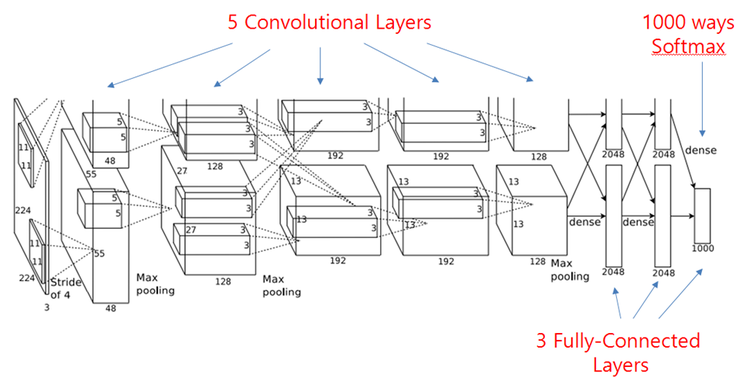
\includegraphics[width=\textwidth]{alexnet2.png}
			\caption{The AlexNet architecture}
			\label{fig:architecture}
		\end{figure}
		The network architecture we decided on is \textit{AlexNet}\cite{alexnet}. Thus, the network contains five convolutional and three fully connected layers. The convolutional layers are followed by max-pooling layers while some dropout layers are placed before the linear layers (see figures \ref{fig:architecture}). An implementation of \textit{AlexNet} is provided by \texttt{PyTorch}. Since the model is suited for images with three color channels we modified the first layer to accept images with only one channel. On the next page, a summary of the network is displayed. It shows, which layers the network contains and how these layers look like.
		\newpage
			\begin{lstlisting}
AlexNet(
  (features): Sequential(
    (0): Conv2d(1, 64, kernel_size=(7, 7), stride=(2, 2),
     padding=(3, 3), bias=False)
    (1): ReLU(inplace)
    (2): MaxPool2d(kernel_size=3, stride=2, padding=0,
     dilation=1, ceil_mode=False)
    (3): Conv2d(64, 192, kernel_size=(5, 5), stride=(1, 1),
     padding=(2, 2))
    (4): ReLU(inplace)
    (5): MaxPool2d(kernel_size=3, stride=2, padding=0,
     dilation=1, ceil_mode=False)
    (6): Conv2d(192, 384, kernel_size=(3, 3), stride=(1, 1),
     padding=(1, 1))
    (7): ReLU(inplace)
    (8): Conv2d(384, 256, kernel_size=(3, 3), stride=(1, 1),
     padding=(1, 1))
    (9): ReLU(inplace)
    (10): Conv2d(256, 256, kernel_size=(3, 3), stride=(1, 1),
     padding=(1, 1))
    (11): ReLU(inplace)
    (12): MaxPool2d(kernel_size=3, stride=2, padding=0,
     dilation=1, ceil_mode=False)
  )
  (avgpool): AdaptiveAvgPool2d(output_size=(6, 6))
  (classifier): Sequential(
    (0): Dropout(p=0.5)
    (1): Linear(in_features=9216, out_features=4096, bias=True)
    (2): ReLU(inplace)
    (3): Dropout(p=0.5)
    (4): Linear(in_features=4096, out_features=4096, bias=True)
    (5): ReLU(inplace)
    (6): Linear(in_features=4096, out_features=15, bias=True)
  )
)
		\end{lstlisting}
		\newpage
		
	\subparagraph{Hyperparameter training}
	The library \texttt{PyTorch} allows to set the training hyper parameters. The ones that are relevant in our routine are the learning rate, the beta values for the \textit{ADAM} optimizer, and the weight decay. To find the optimal values for these parameters, we created a second notebook in which we trained under the same conditions for one epoch with different hyperparameter values and compared the achieved accuracies. Table \ref{tab:hyperparams} shows which values we tried out for each parameter. The best results were achieved with a learning rate of 0.001, a beta tuple of (0.95, 0.95), and a weight decay of 0.
	\begin{table}[h!]
		\begin{tabular}{c|c}
			\textbf{Parameter} & \textbf{Values} \\
			\hline
			Learning rate & 0.01, 0.001, 0.0001 \\
			Beta 1 & 0.8, 0.85, 0.9, 0.95 \\
			Beta 2 & 0.9, 0.925, 0.95, 0.99 \\
			Weight decay & 0, 0.01, 0.001, 0.0001
		\end{tabular}
		\caption{The values we evaluated for the different hyperparameters}
		\label{tab:hyperparams}
	\end{table}
	
	\paragraph{Automatic Classification}
	After the training is complete, we save the model to a \textit{.ckpt} file. The actual classifier that will be used in our program will be an instance of the class \texttt{MathSymbolClassifier}. This class simply contains an \textit{AlexNet} instance in which we load the information from the trained model. To predict what each of our segmented images shows, the class provides a function \texttt{classify}. The function takes a \texttt{NumPy} array with images as an input, creates a tensor out of this array and leads the data through the network. Afterwards the predicted label is returned as a string and can be further processed by the symbolic math solver \texttt{SymPy}.
	
	\paragraph{Manual Classification}
	Before the extracted symbols are given as an input for the automatic classifier, we check manually if they picture a symbol that our classifier can not recognize. This applies for opening and closing brackets, minus symbols, equal signs, commas, and multiplication dots.
	
	\subsection{Calculations}
	\small{Author: Duc Anh Phi} \newline \newline
	
	\section{Experiments}
	\subsection{Comparing Preclassification and Neural Networks}
	\small{Author: Timothy Jay Herbst, Duc Anh Phi} \newline \newline
	In the following experiment we will be testing the Image-Input-Calculator and also give some motivation as to why it uses several preclassification functions.
	For this we will compare how well the calculator performs using three different types of classifiers:\\
	The first classifier is capable of classifying a contour to all symbols that might be in the equation we are analysing.
	Those are the digits "0" through "9","+","-","/", "(" and ")".
	The only time at which we use the preclassification processes are for deciding whether a dot is a multiplication symbols "$\cdot$", a comma "," or dot "." which separates digits larger and smaller than 1 or if the dot is not part of the equation at all.\\
	The second classifier uses as many preclassifying methods as we were able to develop.
	This means it is able to classify a contour to any digit "0" through "9", "+" and both "(" and ")".\\ %??? add accuracy on MNIST and Mixed
	To compare how well they classify, we have created several images of equations with varying amounts of digits.
	Both classifiers have been tested on the same equations and it has been determined, how often a contour was correctly or incorrectly classified.
	These results can be seen in table ??? !!!.
	
	
	%???!!!
	
	When looking at how many equations were correctly classified compared to how long the equation is, one can see ??? !!!
	
	
	
	
	\subsection{Confusion Matrix}
	\small{Author: Fenja Kollasch} \newline \newline
	
	\section{Discussion}
%	In this section, we will discuss the progression of this project regarding the result.
	
	\subsection{Pre-Processing}
	\small{Author: Timothy Jay Herbst} \newline \newline
	Transforming the original image into a usable binary image worked relatively smoothly.
	The main issues which arise during this part are caused by the large variety of images.
	These vary in brightness, background color and medium of writing to name a few.
	However, it was possible to develop a method which consistently gives good results.\\
	The simple pre-processing step performs well on a variety of images.
	It does however, develop problems on very large and small images, because it operates with a fixed kernel size.
	A solution for this would be to have the kernel size adapt with the size of the image or scaling the image.
	However, when scaling the image we found that it could happen that the equation would dissapear if written less clearly.\\
	The border removal process performs well when removing contours caused by objects that are not the equation.
	It does fail sometimes, however, if the colour of the background object does not differ strongly from the background colour.
	Then the border of the object may not be a consistent line.
	It can then not be fully removed and a part of the border may remain (see fig \ref{fig:PartialBorder}).
	\begin{figure*}[htp]
		\centering
		%\subfigure{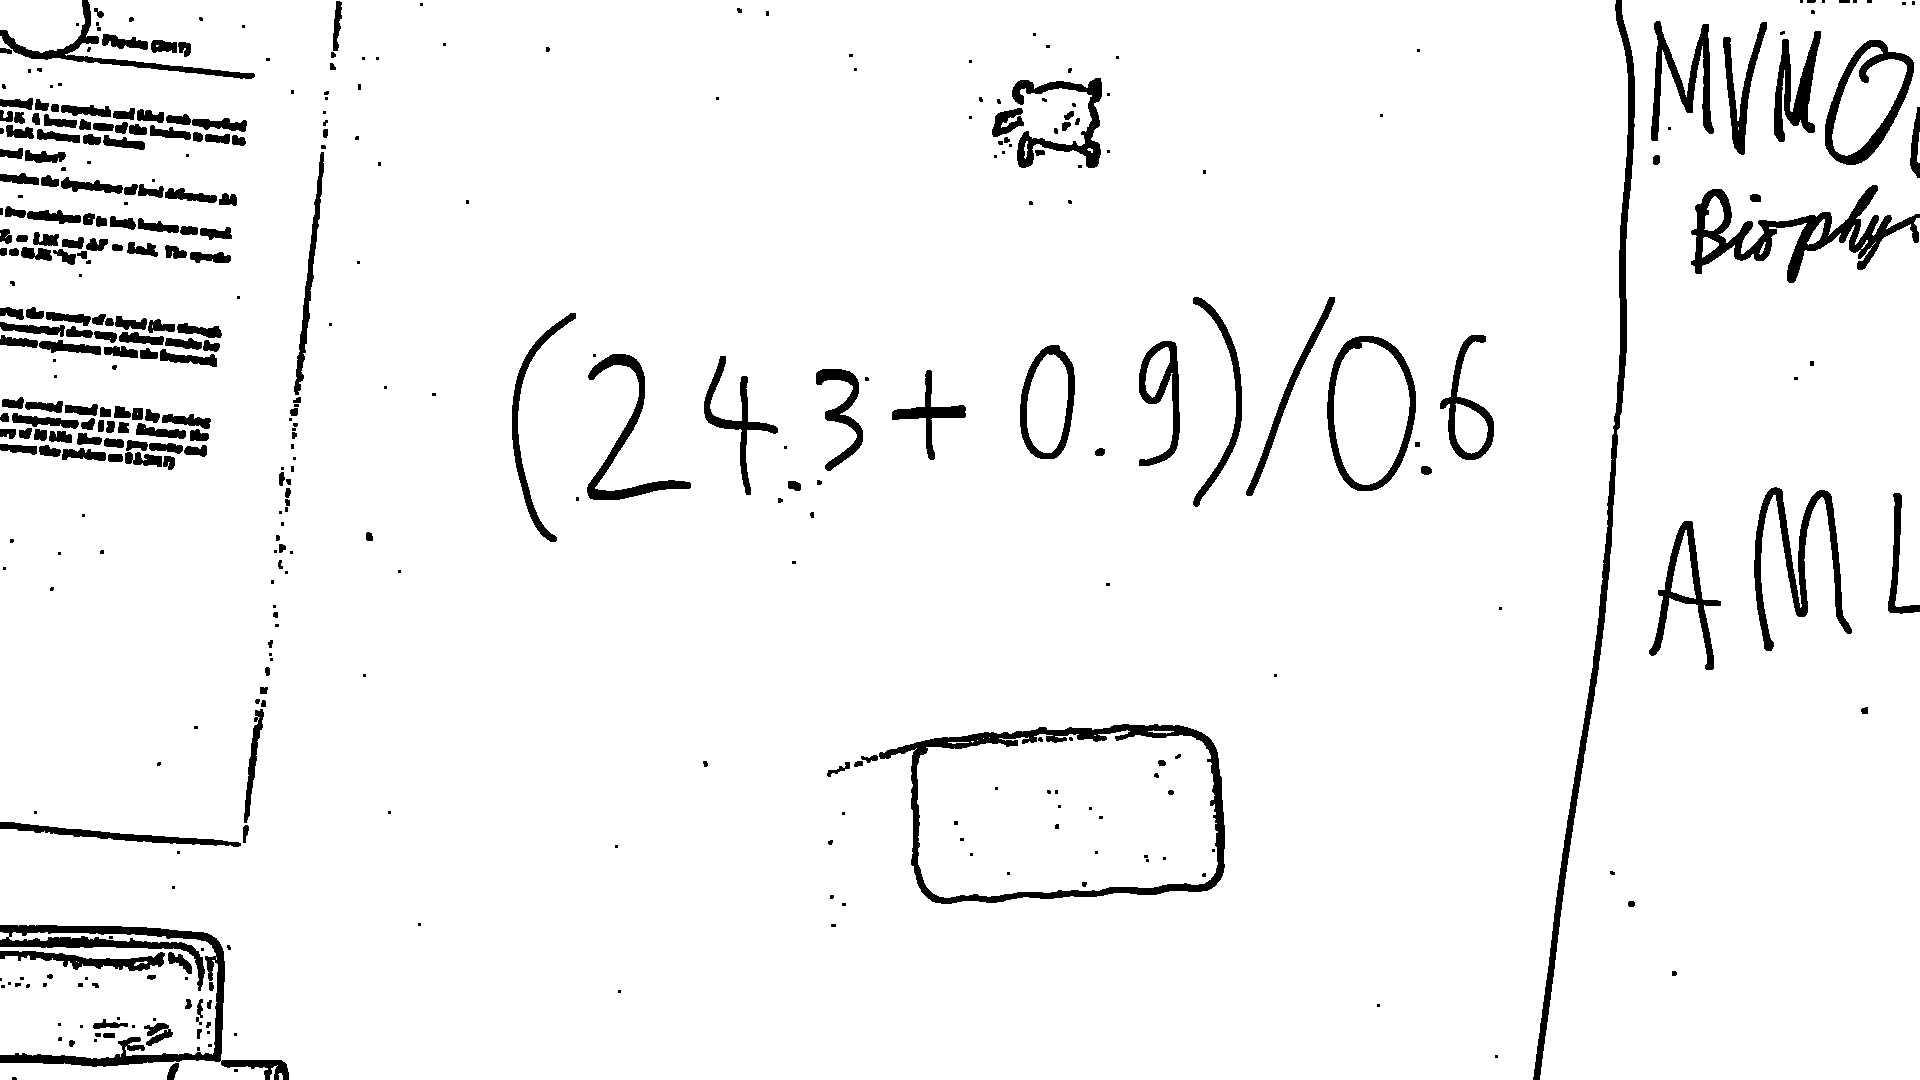
\includegraphics[width=.45\linewidth]{ImagesForReport/PartialBorder1}}\quad
		%\subfigure{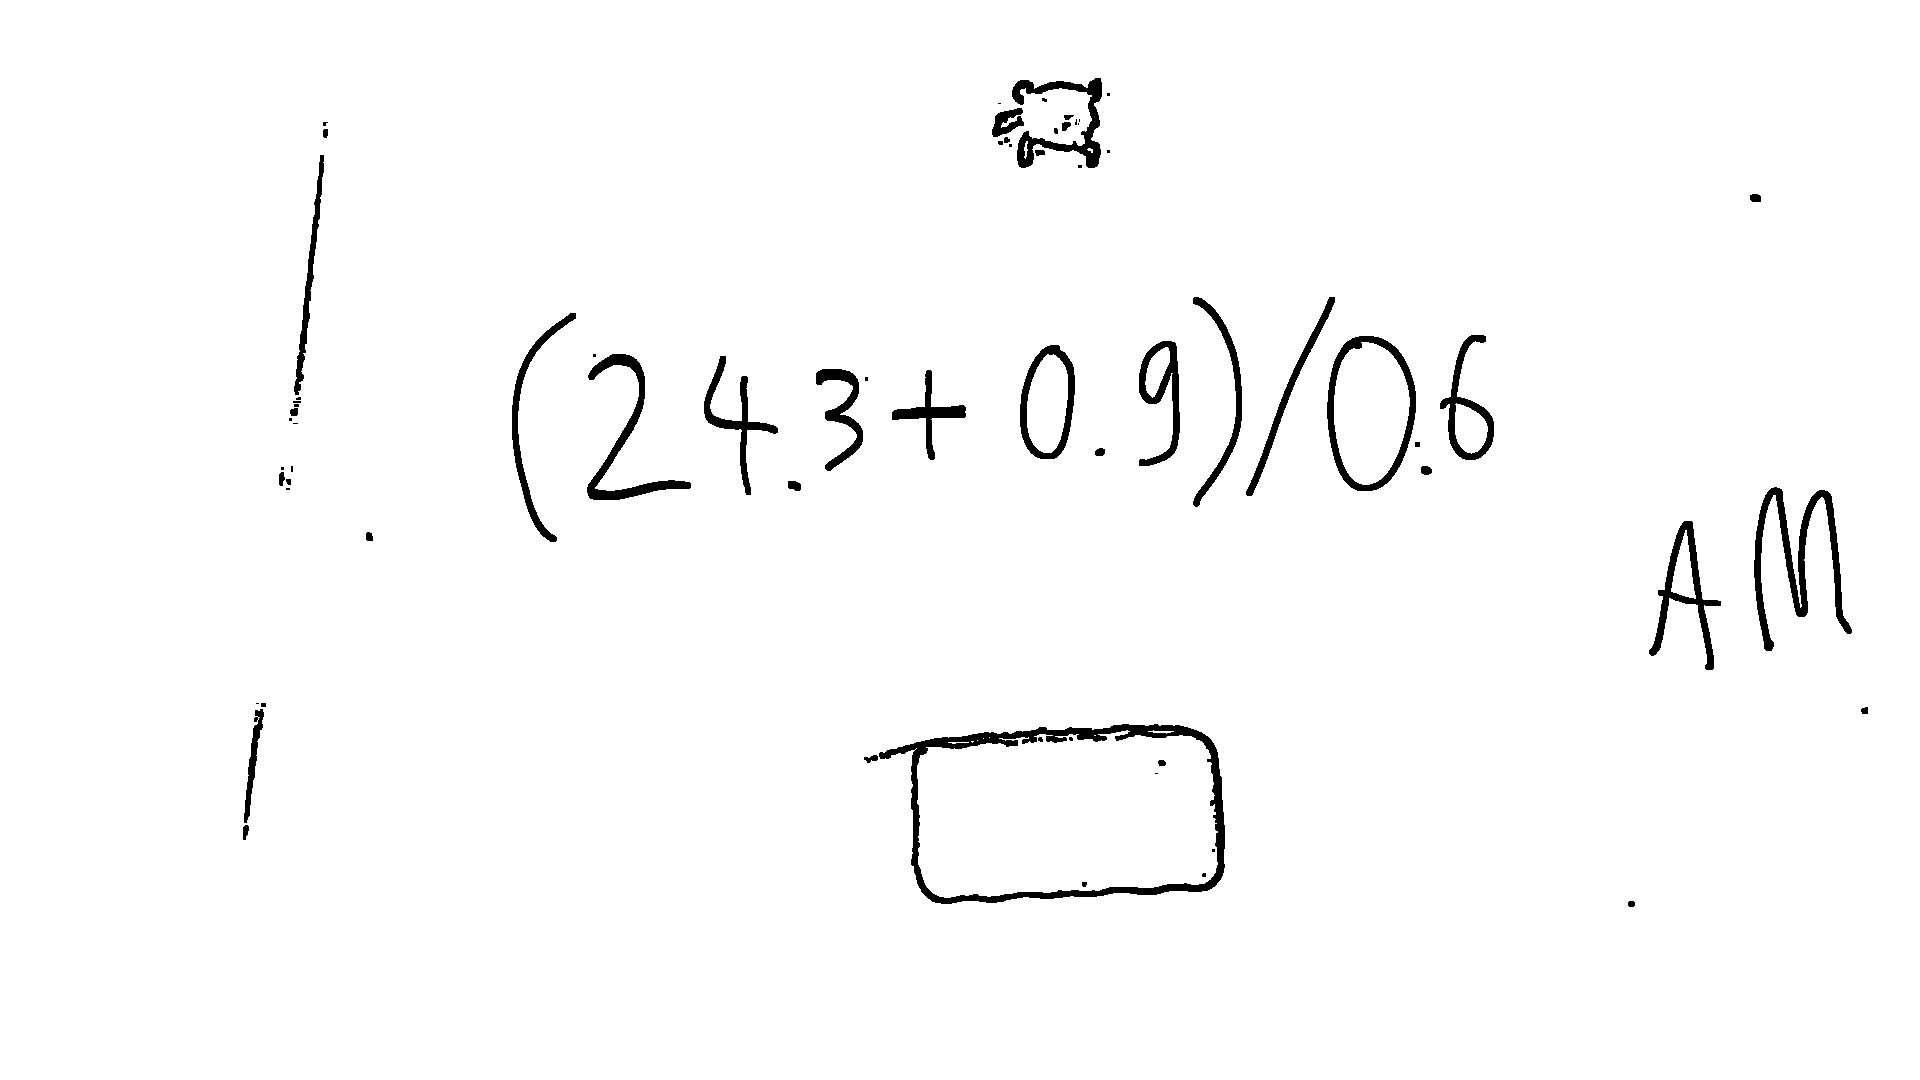
\includegraphics[width=.45\linewidth]{ImagesForReport/PartialBorder2}}
		
		\caption{Many of the background contours are removed.
		However, the paper on the left side of the image is only partially removed and the eraser is to far away from the border to be removed.}
		\label{fig:PartialBorder}
	\end{figure*}
	Also if an object is fully within the image, it is not likely to disappear in this step.
	It will, however, disappear in during the line ordering step because it is the only contour in that line and therefore can't be part of an equation.\\
	
	The brightness removal process allows for the removal of reflected light sources.
	It also helps remove small sources of noise from the background of an image if the background is brighter than the image is on average.
	If the image were on average darker than the equation, it would cause the writing to disappear.
	However, we were never able to observe this on a whiteboard or paper.
	This step makes it impossible to detect an equation on e.g. a blackboard, because here the writing is brighter than the background.
	
	
	
	
	
	
	
	
	
	\subsection{Classification problems}
	\small{Author: Fenja Kollasch} \newline \newline
	A major issue appearing during development was the fact that the usability of our application highly depends on the accuracy of the classifier. Our initial ambition was to recognize various more symbols automatically. Unfortunately, we were not able to gather enough training data and therefore we could not create models with the desired accuracy. Any classifier that recognizes less than 95\% causes major leaks in the overall performance of our program and makes it unusable. Furthermore, it took a long time to create well-trained models what made the training procedure tedious and decelerated our progress.
	
	\subsection{Comparing Preclassification and Neural Networks}
	\small{Author: Timothy Jay Herbst} \newline \newline
	
	\section{Conclusion}
		\small{Author: Timothy Jay Herbst, Fenja Kollasch, Duc Anh Phi} \newline \newline
	The Image-Input-Calculator works reasonably well under difficult circumstances.
	However, it lacks consistency under good circumstances.
	This is particularly problematic considering that a single misclassification will likely produce a wrong result.
	It has difficulties distinguishing between ??? !!!.
	This is due to the difference between simply classifying an image and analysing an image, which may vary quite strongly from the ideal.
	The classifier significantly improved ???!!!check when using certain manual classifications to simplify the possible output of the classifier.
	Another method how the classifier could have improved would be with more training data.
	Even though many online libraries provide a variety of different symbols (which were used), these could only be of so much use, because of the difference between the provided image and a contour which had to undergo the preprocessing steps that are necessary to find the contours.
	On this count, however, the Calculator shines, in that it uses several new methods to detect the significant contours.
	To further improve on this a U-Net ???!!!check could have provided a semantic segmentation between pixels and background.
	
	
	\pagebreak
	\section{Installation and Usage}
	\small{Author: Duc Anh Phi)\\
	\subsection{Installation}
	
	\begin{enumerate}
		\item Install Python 3.6 (if not already installed)
		\item Download the project from \url{https://github.com/DucAnhPhi/image-input-calc}
		\item (Optional) Set up a Python virtual environment for this project. It keeps the dependencies/libraries required by different projects in separate places (isolates them to avoid conflicts). \\
		\\
		Run the following commands in your terminal:
		\begin{verbatim}
		$ pip install virtualenv
		$ cd path/to/image-input-calc
		$ virtualenv -p python3.6 virtual_env
		\end{verbatim}
		To begin using the virtual environment, it needs to be activated.
		\\
		If you are on Linux or MacOS, run the following:

		\begin{verbatim}
		$ source virtual_env/bin/activate
		\end{verbatim}

		If you are on Windows, run the following:

		\begin{verbatim}
		$ virtual_env/Scripts/activate.bat
		\end{verbatim}

		\item Install all project dependencies with:
		\begin{verbatim}
		$ pip install -r requirements.txt
		\end{verbatim}
	\end{enumerate}




\subsection{Usage}
In the project directory, run the program with:

\begin{verbatim}
$ python3 app.py
\end{verbatim}

\newpage
\printbibliography[heading=bibintoc, title={Sources}]
%??? !!! Create bibliography
%	[1] $https://www.tutorialspoint.com/opencv/opencv_adaptive_threshold.htm$ \\
%	[2] $https://docs.opencv.org/2.4/modules/imgproc/doc/miscellaneous_transformations.html?highlight=adaptivethreshold$



%This step had to have a very low false negative rate.
%In other words, we had to allow for a small amount of noise rather than accidently have symbols or parts of symbols disappear.
%The simple pre-processing step performed well on this task.\\
%Images were already usable after preprocessing.
%However, often contours could be found which did not belong to the equation itself.
%These contours can almost always be classified as either objects which are not text (for instance the border of a piece of paper) or as simple noise (caused for instance by the texture of the paper).
%They can be countered for separately.\\

%Unwanted contours caused by background objects are often close to or connect to the border of the image.
%They could often be removed with background removal mask.
%While this often worked, this failed when the colour of the background object does not differ strongly from the background colour.
%This causes the border of the object to be inconsistent which may leave some part of the border in the image.\\

%Contours created by noise tend to be small and appear either statistically isolated or in large clusters.\\
%Isolated pixels of noise are often caused by small aberrations in the texture of the writing medium like paper.\\
%Noisy Pixels which appear in larger groups can often be attributed to reflections of light sources.
%This happens more often on white boards.\\
%Both types offer only minor variations of the brightness of the writing medium and can therefore be countered by using a mask which removes all pixels which are of higher than average brightness in the original image.\\
%While this method is in no way sufficient to detect text, it gives us a fair indicator as to which pixels are not part of the equation.
%This doesn't work if the equation is brighter than the medium it is written on (e.g. a chalk board).
%A simple inversion of the brightness of the original image might be able to solve this problem.
%However, reflected light sources (whose brightness may well be bright than the text) would present a problem.

\end{document}          
